\documentclass{article}

% if you need to pass options to natbib, use, e.g.:
\PassOptionsToPackage{numbers, compress}{natbib}
% before loading nips_2017
%
% to avoid loading the natbib package, add option nonatbib:
% \usepackage[nonatbib]{nips_2017}

\usepackage{nips_2017}

% to compile a camera-ready version, add the [final] option, e.g.:
% \usepackage[final]{nips_2017}

\usepackage[utf8]{inputenc} % allow utf-8 input
\usepackage[T1]{fontenc}    % use 8-bit T1 fonts
\usepackage[colorlinks=true,linkcolor=green,citecolor=cyan]{hyperref}       % hyperlinks
\usepackage{url}            % simple URL typesetting
\usepackage{booktabs}       % professional-quality tables
\usepackage{amsfonts}       % blackboard math symbols
\usepackage{nicefrac}       % compact symbols for 1/2, etc.
\usepackage{microtype}      % microtypography

% My Packages
\usepackage{amsmath}
\usepackage{amssymb}
\usepackage{amsthm}
\usepackage{mathbbol}
\usepackage{mathtools}
\usepackage{mathrsfs}
\usepackage{vector}
\usepackage{cleveref}
\usepackage{bm}
\usepackage[dvipsnames]{xcolor}
\newtheorem{theorem}{Theorem}[section]
\newtheorem{corollary}[theorem]{Corollary}
\newtheorem{lemma}[theorem]{Lemma}
\newtheorem{claim}[theorem]{Claim}
\usepackage{multirow}
\usepackage{algorithm}
\usepackage{algorithmic}

\newcommand{\argmax}{\operatornamewithlimits{argmax}}
\newcommand{\note}[1]{{\color{orange} #1}}
\newcommand{\edit}[1]{{\color{forestgreen} #1}}

\title{CAKE: Classification avec Kernel Embeddings \\ with Rademacher Complexity based Risk Bounds}

% The \author macro works with any number of authors. There are two
% commands used to separate the names and addresses of multiple
% authors: \And and \AND.
%
% Using \And between authors leaves it to LaTeX to determine where to
% break the lines. Using \AND forces a line break at that point. So,
% if LaTeX puts 3 of 4 authors names on the first line, and the last
% on the second line, try using \AND instead of \And before the third
% author name.

\author{
	Kelvin Y.S. Hsu \\
	University of Sydney, Australia\\
	DATA61, CSIRO\\
	\texttt{Kelvin.Hsu@\{sydney.edu.au, data61.csiro.au\}} \\
	%% examples of more authors
	\And
	Richard Nock \\
	Australian National University, Australia\\
	University of Sydney, Australia\\
	DATA61, CSIRO\\
	\texttt{Richard.Nock@data61.csiro.au} \\
	\And
	Fabio T. Ramos \\
	University of Sydney, Australia\\
	DATA61, CSIRO\\
	\texttt{Fabio.Ramos@\{sydney.edu.au, data61.csiro.au\}} \\
	%% \texttt{email} \\
	%% \AND
	%% Coauthor \\
	%% Affiliation \\
	%% Address \\
	%% \texttt{email} \\
	%% \And
	%% Coauthor \\
	%% Affiliation \\
	%% Address \\
	%% \texttt{email} \\
	%% \And
	%% Coauthor \\
	%% Affiliation \\
	%% Address \\
	%% \texttt{email} \\
}

\begin{document}
% \nipsfinalcopy is no longer used

\maketitle

\begin{abstract}
	We propose learning-theoretic bounds for hyperparameter learning of conditional kernel embeddings in the probabilistic multiclass classification context. Kernel embeddings are nonparametric methods to represent probability distributions directly through observed data in a reproducing kernel Hilbert space (RKHS). This property forms the core of modern kernel methods, yet the problem of hyperparameter learning for kernel embeddings remains challenging, often relying on heuristics and domain expertise. We begin by developing the kernel embedding classifier (KEC), and prove the stochastic convergence for its probabilistic inferece. We then prove that its expected classification error can be bounded with high probability using Rademacher complexity based risk bounds. We use this bound to propose a scalable kernel learning algorithm for conditional embeddings with batch stochastic gradient descent. We further apply our proposed kernel learning algorithm to learn feature representations of a deep convolutional network, with improved accuracy as compared to the original network, demonstrating the generality of this approach.
\end{abstract}

\section{Introduction}
\label{sec:introduction}
	
	Kernel embeddings are a principled way to represent probability distributions in a nonparametric setting. By transforming probability distributions into mean embeddings within a reproducing kernel Hilbert space (RKHS), distributions can be represented directly from data without assuming a parametric structure. Consequently, probabilistic inference can be carried out entirely within the RKHS in a nonparametric form, where difficult marginalisation integrals become simple linear algebra operations. This very general and powerful technique is core to modern kernel methods, including support vector machines \citep{scholkopf2002learning}, kernel two-sample testing \citep{gretton2007kernel}, kernel Bayesian inference  \citep{fukumizu2013kernel}, nonparametric density estimation \citep{song2008tailoring, kanagawa2014recovering}, domain-invariant component analysis \citep{muandet2013domain}, dimensionality reduction \citep{fukumizu2004dimensionality}, feature discovery via hypothesis testing \citep{jitkrittum2016interpretable}, and filtering \citep{kanagawa2016filtering}. The problem of estimating the kernel mean in a reproducing kernel Hilbert space (RKHS) is thus central to kernel methods.
	
	Positive definite symmetric kernels $k : \mathcal{X} \times \mathcal{X} \to \mathbb{R}$ are the soul of kernel methods, where they provide a coherent sense of similarity between two elements of the same space through implicitly defining higher dimensional features. However, they are most often selected by design, in which kernel based learning algorithms focus only on learning the weightings on the implicit features, and not the features itself. That is, the kernel itself is not learned. Multiple kernel learning has focused on learning constructions of richer kernels from simpler ones \citep{gonen2011multiple, zien2007multiclass}, although the simpler kernels themselves are also preselected by design. By placing a Gaussian process prior over the function class, Gaussian process models \citep{rasmussen2006gaussian} achieve tractable marginal likelihood based learning algorithms that is able to learn the model hyperparameters, which includes the kernel parameters. However, this approach requires various approximations for non-Gaussian likelihoods, and does not generalise well to non-Gaussian priors. Within the kernel embedding framework itself, hyperparameters has been similarly difficult to tune, and its learning is usually only restricted to heuristical approaches such as cross validation. Recent work has introduced Gaussian process priors on mean embeddings to achieve Bayesian hyperparameter learning \citep{flaxman2016bayesian}. However, the learning is separate from the application domain, and the approach has yet to generalise to conditional embeddings.
	
	In this paper, we take a learning theoretic approach to learn the hyperparameters of a conditional kernel embedding in a supervised manner. We first begin by proposing the kernel embedding classifier (KEC), a principled framework for inferring multiclass probabilistic outputs using conditional embeddings, and provide a proof for its stochastic convergence. We then employ Rademacher complexity as a data dependent model complexity measure, and prove that the expected classification risk can be bounded with high probability by the empirical risk and the trace norm of the conditional embedding. We use this bound to propose a learning objective that learns the balance between performance accuracy and model complexity in a way that does not rely on priors. Finally, we note that the learning algorithm proposed generalises to an one class setting, enabling unsupervised kernel learning on unlabeled data.
	
	Our work also has implications in the supervised learning context. The kernel embedding classifier is natural in the probabilistic multiclass domain. On the other hand, similarly kernel based classifiers such as support vector classifiers (SVC) \citep{m2001introduction} and Gaussian process classifiers (GPC) \citep{rasmussen2006gaussian} are natural only in the binary classification domain, and require extensions to handle the multiclass scenario, such as using one-against-all, one-against-one, or decision trees on multiple independent binary classifiers \citep{aly2005survey, hsu2002comparison}. Moreover, SVCs are not probabilistic by nature, while GPCs are analytically intractable and must resort to posterior approximations. In this paper, we verify the performance and versatility of the kernel embedding classifier on standard UCI datasets. With its generality and flexibility, KECs can also be constructed to learn explicit feature representations, and is inherently compatible with deep neural network type architectures. To this end, we demonstrate that KECs can perform end-to-end learning on a convolutional neural network, while also outperforming the original network.

\section{Hilbert Space Embeddings of Conditional Probability Distributions}
\label{sec:background}

	We begin by providing an overview of Hilbert space embeddings, where probability distributions are represented by mean embeddings in a reproducing kernel Hilbert space (RKHS) through positive definite kernels. Specifically, in the supervised learning context for which we are primarily interested in, we focus on conditional distributions and its representations in the RKHS.
	
	To construct a conditional embedding map $\mathcal{U}_{Y | X}$ corresponding to the distribution $\mathbb{P}_{Y | X}$ where $X : \Omega \to \mathcal{X}$ and $Y: \Omega \to \mathcal{Y}$ are measurable random variables, we choose a kernel $k : \mathcal{X} \times \mathcal{X} \to \mathbb{R}$ for the input space $\mathcal{X}$ and another kernel $l : \mathcal{Y} \times \mathcal{Y} \to \mathbb{R}$ for the output space $\mathcal{Y}$. These kernels $k$ and $l$ each describe how similarity is measured within each of their respective domains $\mathcal{X}$ and $\mathcal{Y}$, and are symmetric and positive definite such that they uniquely define the RKHS $\mathcal{H}_{k}$ and $\mathcal{H}_{l}$. Such a conditional embedding map is then defined by
	\begin{equation}
		\mathcal{U}_{Y | X} := C_{YX} C_{XX}^{-1},
	\label{eq:conditional_embedding}
	\end{equation}
	where $C_{YX} := \mathbb{E}[l(Y, \cdot) \otimes k(X, \cdot)]$ and $C_{XX} := \mathbb{E}[k(X, \cdot) \otimes k(X, \cdot)]$ \citep{song2009hilbert}. The conditional embedding map can be seen as an operator map from $\mathcal{H}_{k}$ to $\mathcal{H}_{l}$. In this sense, it sweeps out a family of conditional embeddings $\mu_{Y | X = x}$ in $\mathcal{H}_{l}$, each indexed by the input variable $x$, via the property $\mu_{Y | X = x} := \mathbb{E}[l(Y, \cdot) | X = x] = \mathcal{U}_{Y | X} k(x, \cdot)$.
	
	Under the assumption that $\mathbb{E}[g(Y) | X = \cdot] \in \mathcal{H}_{k}$, \citet[Theorem 4]{song2009hilbert} proved that the conditional expectation of a function $g \in \mathcal{H}_{l}$ can be expressed as an inner product,
	\begin{equation}
		\mathbb{E}[g(Y) | X = x] = \langle \mu_{Y | X = x}, g \rangle.
	\label{eq:conditional_expectation}
	\end{equation}
	While the assumptions that $\mathbb{E}[g(Y) | X = \cdot] \in \mathcal{H}_{k}$ and $k(x, \cdot) \in \mathrm{image}(C_{XX})$ holds for finite input domains $\mathcal{X}$ for characteristic kernels $k$, it is not necessarily true when $\mathcal{X}$ is a continuous domain \citep{fukumizu2004dimensionality}, which is the scenario for many classification problems. In this case, $C_{YX} C_{XX}^{-1}$ becomes only an approximation to $\mathcal{U}_{Y | X}$, and we instead regularise the inverse and use $C_{YX} (C_{XX} + \lambda I)^{-1}$, which also serves to avoid overfitting \citep[p. 13]{song2013kernel}.
	
	On top of this, in practice we do not have access to the distribution $\mathbb{P}_{X Y}$ to analytically derive the conditional embedding. Instead, we have a finite collection of data points $\{x_{i}, y_{i}\} \in \mathcal{X} \times \mathcal{Y}$, $i \in \mathbb{N}_{n} := \{1, \dots, n\}$, for which the conditional embedding map $\mathcal{U}_{Y | X}$ can be estimated by
	\begin{equation}
		\hat{\mathcal{U}}_{Y | X} = \Psi (K + n \lambda I)^{-1} \Phi^{T},
	\label{eq:empirical_conditional_embedding}
	\end{equation}
	where $K := \{k(x_{i}, x_{j})\}_{i = 1, j = 1}^{n, n}$, $\Phi := \begin{bmatrix} \phi(x_{1}) & \dots & \phi(x_{n}) \end{bmatrix}$, $\Psi := \begin{bmatrix} \psi(y_{1}) & \dots & \psi(y_{n}) \end{bmatrix}$, $\phi(x) := k(x, \cdot)$, $\psi(y) := l(y, \cdot)$, and $\lambda$ is the regularisation parameter for the conditional operator \citep{song2013kernel}. We then define the empirical conditional embedding by $\hat{\mu}_{Y | X = x} := \hat{\mathcal{U}}_{Y | X} k(x, \cdot)$, which stochastically converges to the true conditional embedding $\mu_{Y | X = x}$ in the RKHS norm at a rate of $O_{p}((n \lambda)^{-\frac{1}{2}} + \lambda^{\frac{1}{2}})$, under the assumption that $k(x, \cdot)$ is in the image of $C_{XX}$ \cite[Theorem 6]{song2009hilbert}. This allows us to approximate the conditional expectation \eqref{eq:conditional_expectation} with $\langle \hat{\mu}_{Y | X = x}, g \rangle$ instead, 
	\begin{equation}
		\mathbb{E}[g(Y) | X = x] \approx \langle \hat{\mu}_{Y | X = x}, g \rangle = \bvec{g}^{T} (K + n \lambda I)^{-1} \bvec{k}(x),
	\label{eq:empirical_conditional_expectation}
	\end{equation}
	where $\bvec{g} := \{g(y_{i})\}_{i = 1}^{n}$ and $\bvec{k}(x) := \{k(x_{i}, x\}_{i = 1}^{n}$, knowing that it would converge to the true expectation as $n$ increases for sufficiently small $\lambda$.
	
\section{Kernel Embedding Classifier}
\label{sec:kernel_embedding_classifier}

	In this section, we formulate a kernel embedding based probabilistic classifier by casting it into the conditional embedding framework. In the multiclass setting, the output label space is finite and discrete, taking values only in $\mathcal{Y} = \mathbb{N}_{m} := \{1, \dots, m\}$. Naturally, we first choose the Kronecker delta kernel $\delta : \mathbb{N}_{m} \times \mathbb{N}_{m} \to \{0, 1\}$ as the output kernel $l$, where labels that are the same has unit similarity and labels that are different have no similarity. That is, for all pairs of labels $y_{i}, y_{j} \in \mathcal{Y}$,
	\begin{equation}
		\delta(y_{i}, y_{j}) := \begin{cases}
		1 & \mathrm{if } \quad y_{i} = y_{j}, \\
		0 & \mathrm{otherwise}.
		\end{cases}
	\end{equation}
	As $\delta$ is an integrally strictly positive definite kernel on $\mathbb{N}_{m}$, it is therefore characteristic \citep[Theorem 7]{sriperumbudur2010hilbert}. As such, by definition of characteristic kernels, $\delta$ uniquely defines a RKHS $\mathcal{H}_{\delta}$ \citep{fukumizu2004dimensionality}. Notice that this kernel has no parameters, so that the model hyperparameters only come from the kernel of the input space and the regularisation parameter $\lambda$.
	
	Recall that the RKHS induced by a positive definite kernel is the closure of the span of its kernel induced features \citep{xu2009refinement}, so that $\mathcal{H}_{l} = \overline{\mathrm{span}\{l(y, \cdot) : y \in \mathcal{Y}\}}$. For $\mathcal{Y} = \mathbb{N}_{m}$ and $l = \delta$, this means that any real-valued function $g : \mathbb{N}_{m} \to \mathbb{R}$ that is bounded on its discrete domain $\mathbb{N}_{m}$ is in the RKHS of $\delta$, because we can always write $g = \sum_{y = 1}^{m} g(y) \delta(y, \cdot) \in \mathrm{span}\{\delta(y, \cdot) : y \in \mathcal{Y}\}$.
	
	In particular, indicator functions on $\mathbb{N}_{m}$ are in the RKHS $\mathcal{H}_{\delta}$, since
	\begin{equation}
		\mathbb{1}_{c}(y) := \mathbb{1}_{\{c\}}(y) := \begin{cases}
		1 & \mathrm{if } \quad y \in \{c\} \\
		0 & \mathrm{otherwise}
		\end{cases} = \delta(c, y).
	\label{eq:indicator_function}
	\end{equation}
	That is, indicator functions $\mathbb{1}_{c} = \delta(c, \cdot)$, $c \in \mathbb{N}_{m}$ are simply the canonical kernel features of $\mathcal{H}_{\delta}$. 
	
	While such properties does not becessarily hold for continuous domains in general, this convenient property in the case of a discrete domain $\mathcal{Y}$ with a Kronecker delta kernel $\delta$ is what allows consistent estimations of decision probabilities used in multiclass classification, which we turn to next.
	
	Let $p_{c}(x) := \mathbb{P}[Y = c | X = x]$ be the \textit{decision probability function} for class $c \in \mathbb{N}_{m}$, which is the probability of the class label $Y$ being $c$ when the example $X$ is $x$. We begin by writing this probability as an expectation of indicator functions,
	\begin{equation}
		p_{c}(x) := \mathbb{P}[Y = c | X = x] = \mathbb{P}[Y \in \{c\} | X = x] = \mathbb{E}[\mathbb{1}_{c}(Y) | X = x].
	\label{eq:decision_probability}
	\end{equation}	
	With $\mathbb{1}_{c} \in \mathcal{H}_{\delta}$, we let $g = \mathbb{1}_{c}$ in \eqref{eq:empirical_conditional_expectation} and $\bvec{1}_{c} := \{\mathbb{1}_{c}(y_{i})\}_{i = 1}^{n}$ to estimate the right hand side of \eqref{eq:decision_probability} by
	\begin{equation}
		\hat{p}_{c}(x) = f_{c}(x) := \bvec{1}_{c}^{T} (K + n \lambda I)^{-1} \bvec{k}(x).
	\label{eq:empirical_decision_probability}
	\end{equation}
	Therefore, the vector of empirical decision probability functions over the classes $c \in \mathbb{N}_{m}$ is
	\begin{equation}
		\hat{\bvec{p}}(x) = \bvec{f}(x) := \bvec{Y}^{T} (K + n \lambda I)^{-1} \bvec{k}(x) \in \mathbb{R}^{m},
	\label{eq:empirical_decision_probability_vector}
	\end{equation}
	where $\bvec{Y} := \begin{bmatrix} \bvec{1}_{1} & \bvec{1}_{2} & \cdots & \bvec{1}_{m} \end{bmatrix} \in \{0, 1\}^{n \times m}$ is simply the one hot encoded labels $\{y_{i}\}_{i = 1}^{n}$.

	We proceed to prove that the empirical decision probabilities \eqref{eq:empirical_decision_probability} converges to the true decision probabilities. In fact, the inference distribution \eqref{eq:empirical_decision_probability_vector} is equivalent to a conditional embedding. We direct the reader to the supplementary material for proof.
	\begin{theorem}[Uniform Convergence of Empirical Decision Probability Function]
		\label{thm:probability_convergence_copy}
		Assuming that $k(x, \cdot)$ is in the image of $C_{XX}$, the empirical decision probability function $\hat{p}_{c} : \mathcal{X} \to \mathbb{R}$ \eqref{eq:empirical_decision_probability} converges uniformly to the true decision probability $p_{c} : \mathcal{X} \to [0, 1]$ \eqref{eq:decision_probability} at a stochastic rate of at least $O_{p}((n \lambda)^{-\frac{1}{2}} + \lambda^{\frac{1}{2}})$ for all $c \in \mathcal{Y} = \mathbb{N}_{m}$.
	\end{theorem}
	While decision probability estimates \eqref{eq:empirical_decision_probability} do not necessarily form a normalised distribution for finite $n$, \cref{thm:probability_convergence_copy} guarantees that they approach one with increasing sample sizes. If normalised distributions are required for interpretation, distribution estimates \eqref{eq:empirical_decision_probability} can be clip-normalised,
	\begin{equation}
		\tilde{p}_{c}(x) := \frac{\max\{\hat{p}_{c}(x), 0\}}{\sum_{j = 1}^{m} \max\{\hat{p}_{j}(x), 0\}}.
	\label{eq:empirical_decision_probability_clip_normalised}
	\end{equation}
	Of course, classification $\hat{y}(x) = \argmax_{c \in \mathbb{N}_{m}} \hat{p}_{c}(x) = \argmax_{c \in \mathbb{N}_{m}} \tilde{p}_{c}(x)$ remains invariant.  \Cref{thm:probability_convergence_copy} also implies the reducing effect of clip-normalisation as with increasing sample sizes, where $\tilde{p}_{c}(x)$ approaches to both $\hat{p}_{c}(x)$ and $p_{c}(x)$.
	
\section{Hyperparameter Learning with Rademacher Complexity Bounds}
\label{sec:hyperparameter_learning}

	Kernel embedding classifiers are equivalent to a conditional embedding with a discrete target space $\mathcal{Y}$. We now turn to address hyperparameter learning for the KEC, and explicitly denote the kernel parameters $\theta \in \Theta$ and regularisation parameter $\lambda \in \Lambda = \mathbb{R}_{+}$ that define the KEC model. Hyperparameter learning for conditional embeddings is particularly difficult compared to joint embeddings, since the kernel $\{k_{\theta} : \theta \in \Theta\}$ is to be learned jointly with a regularisation parameter $\lambda$.  While the conditional embedding map $\hat{\mathcal{U}}_{Y | X}$ \eqref{eq:empirical_conditional_embedding} is the operator $\mathcal{U}$ that minimises the regularised least squares loss $\frac{1}{n} \sum_{i = 1}^{n} \| \psi(y_{i}) - \mathcal{U} \phi(x_{i}) \|_{\mathcal{H}_{l}}^{2} + \lambda \| \mathcal{U} \|_{HS}$ in the RKHS \citep{song2013kernel}, minimising this loss directly over $\theta \in \Theta, \lambda \in \Lambda$ for $\mathcal{U} = \hat{\mathcal{U}}^{(\theta, \lambda)}_{Y | X}$ would trivially result in an overfitted model with $\lambda \rightarrow 0$. This implies that the notion of model complexity is especially important. Nevertheless, current standard solutions employ either cross validation or nested loops separating $\theta$ and $\lambda$, both of which are heuristics and subject to design choices.
	
	To this end, we propose to use a learning theoretic approach to quantify a balance between model complexity and performance accuracy.  The Rademacher complexity \citep{bartlett2002rademacher} measures the expressiveness of a function class $F$ by its ability to shatter, or fit, noise. They are data-dependent measures, and are thus particularly well suited to learning tasks where generalisation ability is vital, since complexity penalties that are not data dependent cannot be universally effective \citep{kearns1997experimental}. 
	
	We begin by defining a loss function as a measure for the generalisation error. For decision functions of the form $\bvec{f} : \mathcal{X} \to \mathcal{A} = \mathbb{R}^{m}$ where entries of $f$ are interpreted as probabilities, we employ the cross entropy loss,
	\begin{equation}
		\mathcal{L}_{\epsilon}(y, \bvec{f}(x)) := - \log{ [\bvec{y}^{T} \bvec{f}(x)]_{\epsilon}^{1} } = - \log{ [f_{y}(x)]_{\epsilon}^{1} },
	\label{eq:cross_entropy_loss_copy}
	\end{equation}
	to express classification risk, where we use the notation $[\;\cdot\;]_{\epsilon}^{1} := \min\{\max\{\;\cdot\;, \epsilon\}, 1\}$. Under this loss, we prove that the expected risk for the kernel embedding classifier $\bvec{f} = \bvec{f}_{\theta, \lambda}$ \eqref{eq:empirical_decision_probability_vector} is bounded by the empirical risk and a Rademacher complexity bound $r(\theta, \lambda)$ with high probability. We refer the reader to the supplementary material for detailed proof.
	
	\begin{theorem}[Expected Risk Bound for KEC Hyperparameter Learning]
		\label{thm:expected_risk_bound_hyperparameter_learning_copy}
		
		For any integer $n \in \mathbb{N}_{+}$ and any set of training observations $\{x_{i}, y_{i}\}_{i = 1}^{n}$ used to define $\bvec{f}_{\theta, \lambda}$ \eqref{eq:empirical_decision_probability_vector}, with probability $1 - \beta$ over \textit{iid} samples $\{X_{i}, Y_{i}\}_{i = 1}^{n}$ of length $n$ from $\mathbb{P}_{X Y}$, every $\theta \in \Theta$, $\lambda \in \Lambda$, and $\epsilon \in (0, e^{-1})$ satisfies
		\begin{equation}
			\mathbb{E}[\mathcal{L}_{e^{-1}}(Y, \bvec{f}_{\theta, \lambda}(X))] \leq \frac{1}{n} \sum_{i = 1}^{n} \mathcal{L}_{\epsilon}(Y_{i}, \bvec{f}_{\theta, \lambda}(X_{i})) + 4 e r(\theta, \lambda) + \sqrt{\frac{8 \log{\frac{2}{\beta}}}{n}},
		\label{eq:expected_risk_bound_hyperparameter_learning_copy}
		\end{equation}
		where $r(\theta, \lambda) := \sqrt{\mathrm{trace}\bigg(\bvec{Y}^{T} (K_{\theta} + n \lambda I)^{-1} K_{\theta} (K_{\theta} + n \lambda I)^{-1} \bvec{Y}\bigg) \sup_{x \in \mathcal{X}} k_{\theta}(x, x)}$.
	\end{theorem}
	
	\begin{algorithm}[tb]
		\caption{KEC Hyperparameter Learning with Batch Stochastic Gradient Descent}
		\label{alg:kernel_embedding_classifier_training}
		\begin{algorithmic}[1]
			\STATE {\bfseries Input:} kernel family $k_{\theta} : \mathcal{X} \times \mathcal{X} \to \mathbb{R}$, dataset $\{x_{i}, y_{i}\}_{i = 1}^{n}$, initial kernel parameters $\theta_{0}$, initial regularisation parameter $\lambda_{0}$, learning rate $\eta$, gradient error tolerance $\epsilon$, batch size $n_{b}$
			\STATE $\theta \leftarrow \theta_{0}$, $\lambda \leftarrow \lambda_{0}$
			\REPEAT
			\STATE Sample the next batch $\mathcal{I} \subseteq \mathbb{N}_{n}$, $| \mathcal{I} | = n_{b}$ \hspace{\fill} (For gradient descent, $n_{b} = n$ and $\mathcal{I} = \mathbb{N}_{n}$)
			\STATE $Y \leftarrow \{\delta(y_{i}, c) : i \in \mathcal{I}, c \in \mathbb{N}_{m}\} \hspace{\fill} \in \{0, 1\}^{n_{b} \times m}$
			\STATE $K_{\theta} \leftarrow \{k_{\theta}(x_{i}, x_{j}) : i \in \mathcal{I}, j \in \mathcal{I}\} \hspace{\fill} \in \mathbb{R}^{n_{b} \times n_{b}}$
			\STATE $L_{\theta, \lambda} \leftarrow \mathrm{cholesky}(K_{\theta} + n_{b} \lambda I_{n_{b}}) \hspace{\fill} \in \mathbb{R}^{n_{b} \times n_{b}}$
			\STATE $V_{\theta, \lambda} \leftarrow L_{\theta, \lambda}^{T} \backslash (L_{\theta, \lambda} \backslash Y) \hspace{\fill} \in \mathbb{R}^{n_{b} \times m}$
			\STATE $P_{\theta, \lambda} \leftarrow K_{\theta} V_{\theta, \lambda} \hspace{\fill} \in \mathbb{R}^{n_{b} \times m}$
			\STATE $q(\theta, \lambda) \leftarrow \frac{1}{n} \sum_{i = 1}^{n} \mathcal{L}_{\epsilon}((Y)_{i}, (P_{\theta, \lambda})_{i}) + 4 e \alpha(\theta) \sqrt{\mathrm{trace}(V_{\theta, \lambda}^{T} K_{\theta} V_{\theta, \lambda})}$
			\STATE $\theta \leftarrow \theta - \eta \frac{\partial q}{\partial \theta}(\theta, \lambda)$, $\lambda \leftarrow \lambda - \eta \frac{\partial q}{\partial \lambda}(\theta, \lambda)$ \hspace{\fill} (Or other gradient based updates such as Adam)
			\UNTIL{$\big\lVert \begin{bmatrix} \frac{\partial q}{\partial \theta}(\theta, \lambda)^{T} & \frac{\partial q}{\partial \lambda}(\theta, \lambda)^{T} \end{bmatrix}^{T} \big\rVert_{\infty} < \epsilon$} \hspace{\fill} (Stop if magnitude of all gradients are below $\epsilon$)
			\STATE {\bfseries Output:} kernel parameters $\theta$, regularisation parameter $\lambda$
		\end{algorithmic}
	\end{algorithm}
	
	In order for the bound \eqref{eq:expected_risk_bound_hyperparameter_learning_copy} to be non-trivial, we focus on bounded kernels in the sense that $\alpha^{2}(\theta) := \sup_{x \in \mathcal{X}} k_{\theta}(x, x) < \infty$. For example, Gaussian kernels $k_{\theta}(x, x') = \sigma_{f}^{2} \exp{( - \frac{1}{2}(x - x') \Sigma^{-1} (x - x') )}$ and similar stationary kernels such as the Mat\'{e}rn family with sensitivity and length scales $\theta = (\sigma_{f}, \Sigma)$ have $\alpha(\theta) = \sigma_{f}$. For non-stationary kernels such as the linear or polynomial kernels, the domain $\mathcal{X}$ is assumed to be compact and thus can be rescaled so that $\alpha(\theta) = 1$. Since the training set itself is a sample of length $n$ drawn from $\mathbb{P}_{X Y}$, the inequality \eqref{eq:expected_risk_bound_hyperparameter_learning_copy} is true with probability $1 - \beta$ when the random variables $X_{i}, Y_{i}$ are realised as the training observations $x_{i}, y_{i}$. We therefore employ this upper bound as the hyperparameter learning objective,
	\begin{equation}
		q(\theta, \lambda) := \frac{1}{n} \sum_{i = 1}^{n} \mathcal{L}_{\epsilon}(y_{i}, \bvec{f}_{\theta, \lambda}(x_{i})) + 4 e r(\theta, \lambda).
	\label{eq:learning_objective}
	\end{equation}
	We employ gradient based optimisers such as Gradient descent or Adam \citep{kingma2014adam}. Since \cref{thm:expected_risk_bound_hyperparameter_learning_copy} holds for any $n \in \mathbb{N}_{+}$ and any set of training data $\{x_{i}, y_{i}\}_{i = 1}^{n}$, with the trade-off of relaxing the bound tightness through $\sqrt{8 \log{(2 / \beta)} / n}$, the bound \eqref{eq:expected_risk_bound_hyperparameter_learning_copy} also holds with high probability for a batch subset of the training data. This enables scalable kernel learning through batch stochastic gradient updates, where each gradient update stochastically attempts to minimise a different upper bound of the generalisation risk. Because this upper bound holds with high probability over \textit{iid} samples, through randomly selecting the \textit{iid} samples used to compute the upper bound, with the same high probability the resulting stochastic gradient will attempt to minimise a strict upper bound. We present this scalable kernel learning via batch stochastic gradient updates in \cref{alg:kernel_embedding_classifier_training}, reducing the time complexity from $O(n^{3})$ to $O(n_{b}^{3})$, where $n_{b}$ is the batch size.
	
	NEED TO SHOW VISUALISATIONS OF SPIRAL HERE AND DISCUSS TWO INITIALISATIONS: ONE OVERFITTING AND ONE UNDERFITTING, AND SHOW THAT OUR TRAINING ALGORITHM FINDS A BALANCE FROM BOTH INITIAL SETTINGS.
	
	ALSO SHOW REVERSE EMBEDDING RESULTS
	
	\textbf{Neural Network Kernels.} DISCUSSION NOT DONE
	


\section{Related Work}
\label{sec:related_work}

	For a linear class of predictors parametrised as $f(x; W) = W^{T} x$, $W \in \mathbb{R}^{d \times L}$, \cite{yu2014large} used trace norm regularisation to bound the Rademacher complexity, achieving tight generalisation bounds in the context of multi-label learning. The KEC predictor \eqref{eq:empirical_decision_probability_vector} has the same linear form in the feature space, $\bvec{f}_{\theta, \lambda}(x) = \bvec{Y}^{T} (K_{\theta} + n \lambda I)^{-1} \Phi_{\theta}^{T} \phi_{\theta}(x) = \hat{\mathcal{U}}^{(\theta, \lambda)}_{Y | X} \phi_{\theta}(x)$, where instead of learning the operator $W^{T}$ directory, we learn hyperparameters $\theta \in \Theta, \lambda \in \Lambda$ for the empirical conditional embedding map $\mathcal{U}^{(\theta, \lambda)}_{Y | X}$ to learn the features $\phi_{\theta}(x)$. \cite{xu2016local} extends the trace norm regularisation approach by considering the local Rademacher complexity on a subset of the predictor class, where they instead minimise the tail sum of the predictor singular values. In the proof of \cref{thm:expected_risk_bound_hyperparameter_learning_copy}, $\theta \in \Theta$ and $\lambda \in \Lambda$ define subsets of $\Theta$ and $\Lambda$ where the Rademacher complexity is considered over. By minimising $q(\theta, \lambda)$, we shrink the subset being considered, achieving localised Rademacher complexity based feature learning without selecting parameters that define the tail sum. Local Rademacher complexity has also been employed for multiple kernel learning \citep{kloft2011local, cortes2013learning} to learn convex combinations of simpler kernels for a support vector machine. We extend its application to the probabilistic multiclass case, and use Rademacher complexity based risk bounds to learn the hyperparameters of a conditional kernel embedding.

	DISCUSSION NOT DONE
	
\section{Experiments}
\label{sec:experiments}

	We demonstrate the average performance of learning anisotropic Gaussian kernels and fully connected neural network kernels under the kernel embedding classification framework on standard UCI datasets, summarised in \cref{tab:stationary_experiments}. The former has a shallow but wide model architecture, while the latter has a deeper but narrower model architecture.
	
	The Gaussian kernel is learned through both the original gradient update (GKEC) and the scalable batch stochastic gradient update (GKEC-SGD) using a tenth ($n_{b} \approx \frac{n}{10}$) of the training set each time, with sensitivity and length scales initialised to $1$. For neural network kernels, we randomly select two simple fully connected architectures with 16-32-8 (NNKEC-1) and 96-32 (NNKEC-2) hidden units respectively, and learn the corresponding kernel without dropout under ReLU activation. Weight parameters are initialised from a truncated normal distribution with standard deviation $0.1$, while biases are initialised to $0.1$, and are to be trained with full gradient updates. For all experiments, regularisation parameter $\lambda$ is initialised to $1$ and is learned jointly with the kernel. Classifiers are trained with the Adam optimiser \citep{kingma2014adam} in TensorFlow \citep{abadi2016tensorflow} with a learning rate of $\eta = 0.1$ and $\epsilon = 10^{-15}$ for learning objective $q(\theta, \lambda)$. Training is ran for 1000 or 10000 iterations when using full or batch stochastic gradient updates respectively, regardless of training convergence. All datasets are scaled so that all dimensions are in the unit range. Each classifier is trained on 9 out of 10 folds and tested on the remaining fold. The folds are shuffled over all 10 combinations to obtain the average test accuracy. We also provide typical performance on the dataset using other approaches. See supplementary material for details. These numbers are only illustrative, however, in that other work may have used different data pre-processing, folds, or longer training time. 
	
	- \texttt{banknote}: ANN: 99.78 \citep{kaya2016banknote} \\
	- \texttt{ecoli}: Probabilistic Binary Tree: 81.1 \citep{horton1996probabilistic} \\
	- \texttt{robot}: ANN: 97.6 \citep{freire2009short} \\
	- \texttt{segment}: Decision Trees \& Neural Nets: 99.14 - 99.98 \citep{lim2000comparison} \\
	- \texttt{wine}: RDA: 100, QDA: 99.4, LDA: 98.9, 1NN: 96.1 \citep{aeberhard1992comparison} \\
	- \texttt{yeast}: Probabilistic Binary Tree: 55.0 \citep{horton1996probabilistic} \\
	
	STILL HAS TO ADD CONVOLUTIONAL KERNEL MNIST STUFF WHICH ACHIEVED 99.5\% TEST ACCURACY WITH SGD
	
	ALSO SHOW REVERSE EMBEDDING RESULTS TO OBTAIN THE CLASS MODES
	
	DISCUSSION NOT DONE 
%	\begin{table}[t]
%		\begin{center}
%			\begin{tabular}{ l | c | c }
%				\hline
%				\multicolumn{3}{ c }{Classification Accuracy on UCI Datasets} \\
%				\hline
%				\hline				
%				Dataset \hspace{\fill} $(n, d, m)$ & Method & Test Accuracy \\
%				\hline
%				\hline
%				\texttt{banknote} & Gaussian KEC & $99.93 \pm 0.22$ \\
%				(1372, 4, 2) & Gaussian KEC (SGD 124) & $98.83 \pm 0.88$ \\
%				& Neural KEC (16, 32, 8) & $99.49 \pm 1.03$ \\
%				& Neural KEC (96, 32) & $99.42 \pm 0.91$ \\
%				\hline
%				\texttt{ecoli} & Gaussian KEC & $87.50 \pm 4.36$ \\
%				(336, 7, 8) & Gaussian KEC (SGD 30) & $84.50 \pm 5.02$ \\
%				& Neural KEC (16, 32, 8) & $87.49 \pm 3.24$ \\
%				& Neural KEC (96, 32) & $86.32 \pm 5.98$ \\
%				\hline
%				\texttt{robot} & Gaussian KEC & \\
%				(5456, 24, 4) & Gaussian KEC (SGD 491) & $95.45 \pm 0.86$ \\
%				& Neural KEC (16, 32, 8) & $82.31 \pm 7.11$ \\	
%%				\texttt{robot} \hspace{\fill} (5456, 24, 4) & Neural KEC (96, 32) & $92.25 \pm 1.39$ \\	
%				& Neural KEC (96, 32) & $94.50 \pm 0.75$ \\
%				\hline
%				\texttt{segment} & Gaussian KEC & \\
%				(2310, 19, 7) & Gaussian KEC (SGD 208) & $96.10 \pm 1.46$ \\
%				& Neural KEC (16, 32, 8) & $94.59 \pm 1.62$ \\
%				& Neural KEC (96, 32) & $96.71 \pm 1.06$ \\
%				\hline
%				\texttt{wine} & Gaussian KEC & $97.22 \pm 3.73$ \\
%				(178, 13, 3) & Gaussian KEC (SGD 16) & $93.27 \pm 6.04$ \\
%				& Neural KEC (16, 32, 8) & $96.11 \pm 5.00$\\
%				& Neural KEC (96, 32) & $97.22 \pm 5.12$ \\
%				\hline
%				\texttt{yeast} & Gaussian KEC & $52.49 \pm 2.06$ \\
%				(1484, 8, 10) & Gaussian KEC (SGD 134) & $60.30 \pm 4.39$ \\
%				& Neural KEC (16, 32, 8) & $55.80 \pm 4.96$ \\
%				& Neural KEC (96, 32) & $59.57 \pm 3.98 $ \\
%				\hline
%				\hline
%			\end{tabular}
%		\end{center}
%		\caption{Classification accuracy of two kernel embedding classification architectures on standard UCI Datasets. Numbers after ``SGD'' indicates the batch size used. Numbers after ``Neural KEC'' indicates the size of the hidden layers, starting from the first.}
%		\label{tab:stationary_experiments_old}
%	\end{table}
		
	\begin{table}[t]
		\caption{Classification accuracy of Gaussian and Neural Network KEC on UCI datasets}
		\label{tab:stationary_experiments}
		\centering
		\begin{tabular}{lccccc}			
			Dataset \hspace{\fill} $(n, d, m)$ & GKEC & GKEC-SGD & NNKEC-1 & NNKEC-2 & Others \\
			\midrule
			\texttt{banknote} \hspace{\fill} (1372, 4, 2) & $99.9 \pm 0.2$ & $98.8 \pm 0.9$ & $99.5 \pm 1.0$ & $99.4 \pm 0.9$ & 99.78 \\
			\texttt{ecoli} \hspace{\fill} (336, 7, 8) & $87.5 \pm 4.4$ & $84.5 \pm 5.0$ & $87.5 \pm 3.2$ & $86.3 \pm 6.0$ & 81.1 \\
			\texttt{robot} \hspace{\fill} (5456, 24, 4) & $97.8$ & $95.5 \pm 0.9$ & $82.3 \pm 7.1$ & $94.5 \pm 0.8$ & 97.59 \\
			\texttt{segment} \hspace{\fill} (2310, 19, 7) & $98.4 \pm 0.8$ & $96.1 \pm 1.5$ & $94.6 \pm 1.6$ & $96.7 \pm 1.1$ & 99.14 \\
			\texttt{wine} \hspace{\fill} (178, 13, 3) & $97.2 \pm 3.7$ & $93.3 \pm 6.0$ & $96.1 \pm 5.0$ & $97.2 \pm 5.1$ & 98.9 \\
			\texttt{yeast} \hspace{\fill} (1484, 8, 10) & $52.5 \pm 2.1$ & $60.3 \pm 4.4$ & $55.8 \pm 5.0$ & $59.6 \pm 4.0$ & 55.0 \\
		\end{tabular}
	\end{table}



	\begin{figure}[t]
		\centering
		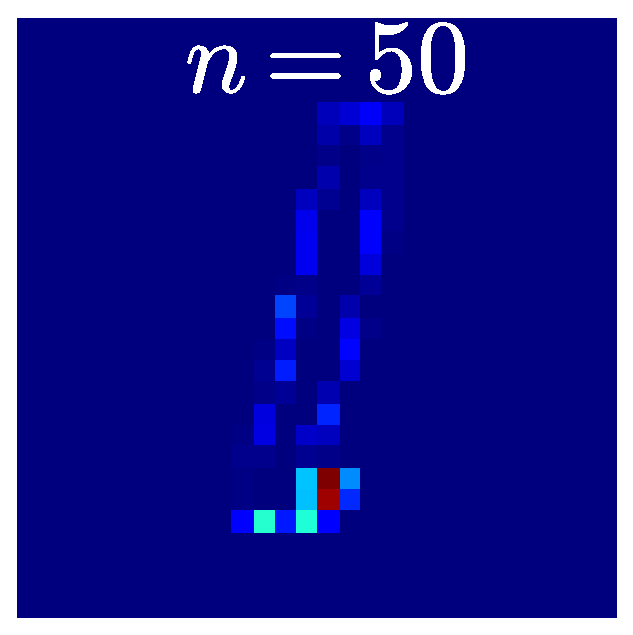
\includegraphics[width=0.1\linewidth]{figures/pixel_relevance_50.eps}
		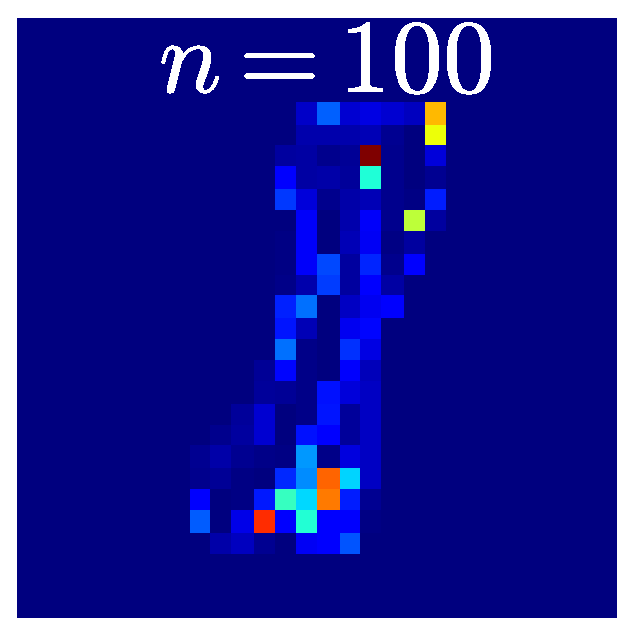
\includegraphics[width=0.1\linewidth]{figures/pixel_relevance_100.eps}
		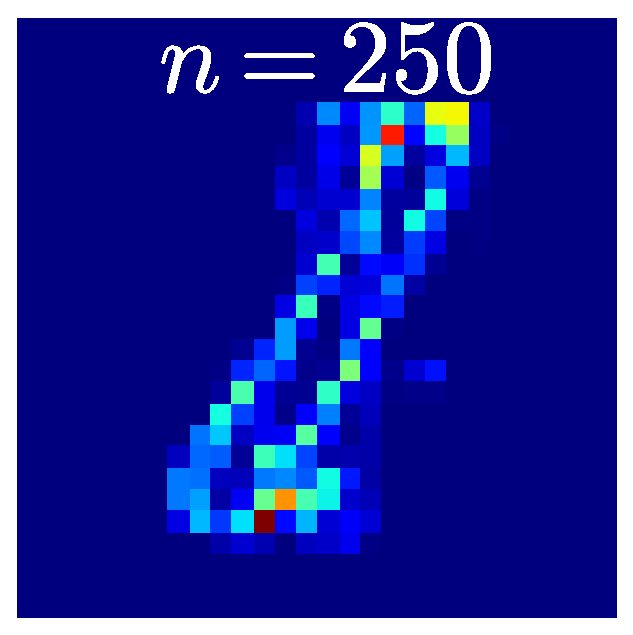
\includegraphics[width=0.1\linewidth]{figures/pixel_relevance_250.eps}
		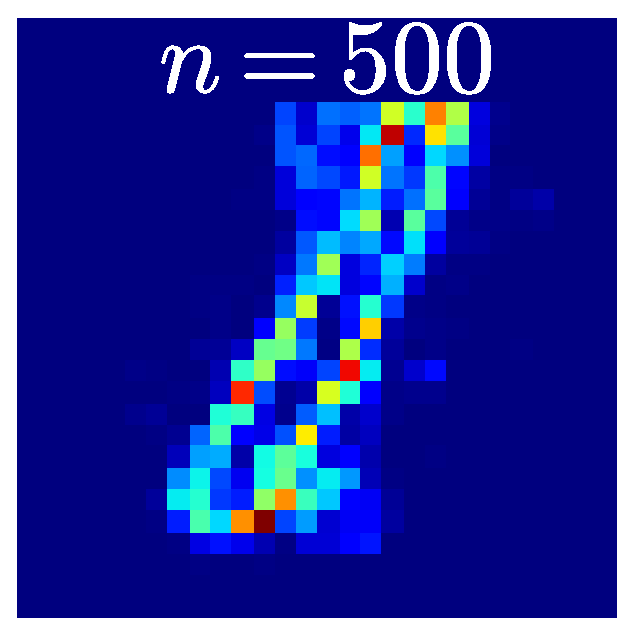
\includegraphics[width=0.1\linewidth]{figures/pixel_relevance_500.eps}
		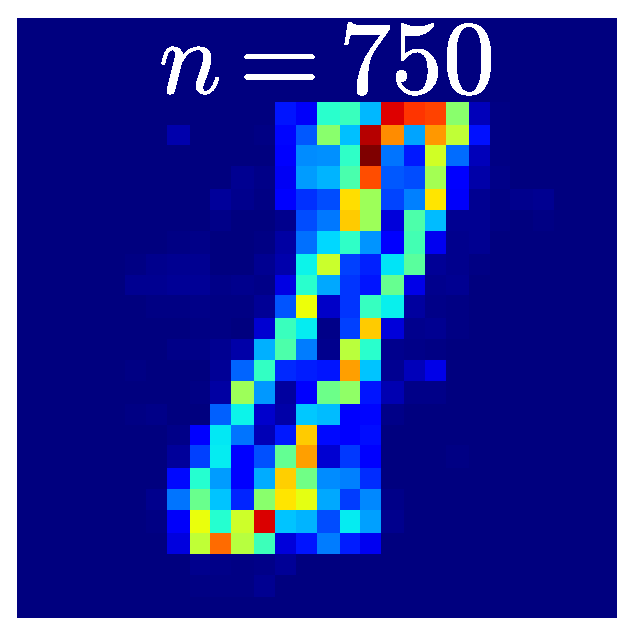
\includegraphics[width=0.1\linewidth]{figures/pixel_relevance_750.eps}
		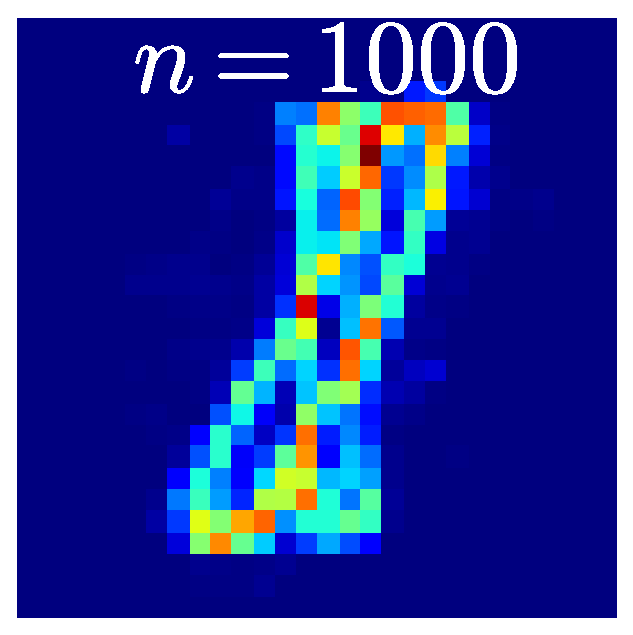
\includegraphics[width=0.1\linewidth]{figures/pixel_relevance_1000.eps}
		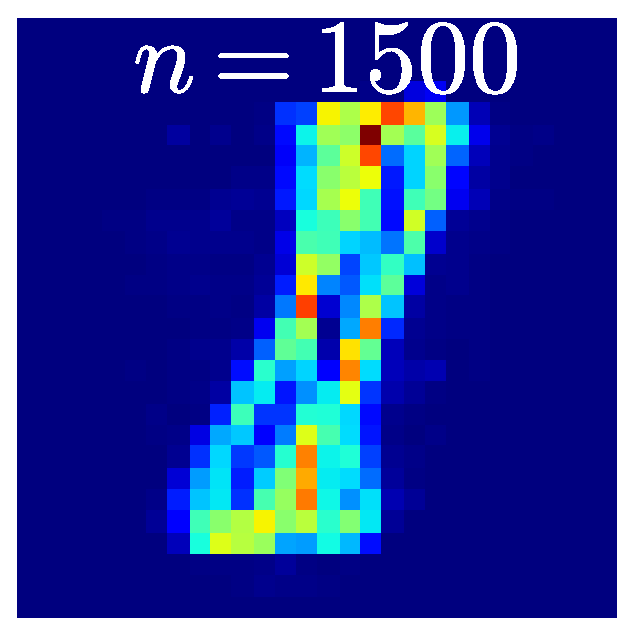
\includegraphics[width=0.1\linewidth]{figures/pixel_relevance_1500.eps}
		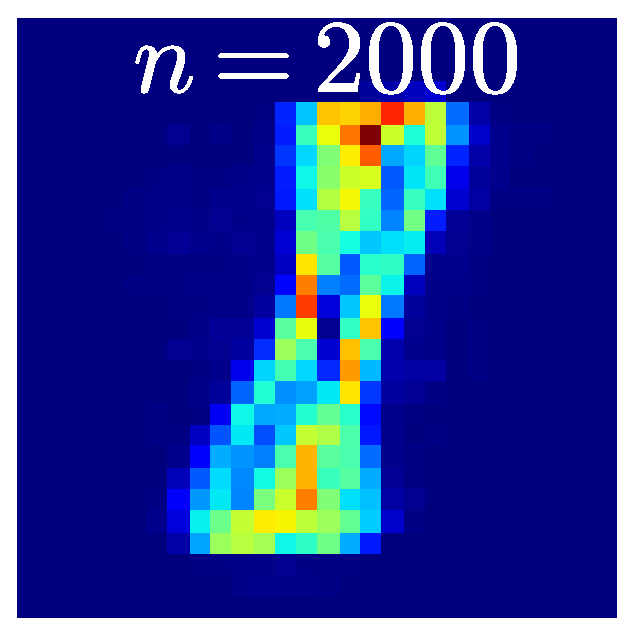
\includegraphics[width=0.1\linewidth]{figures/pixel_relevance_2000.eps}
		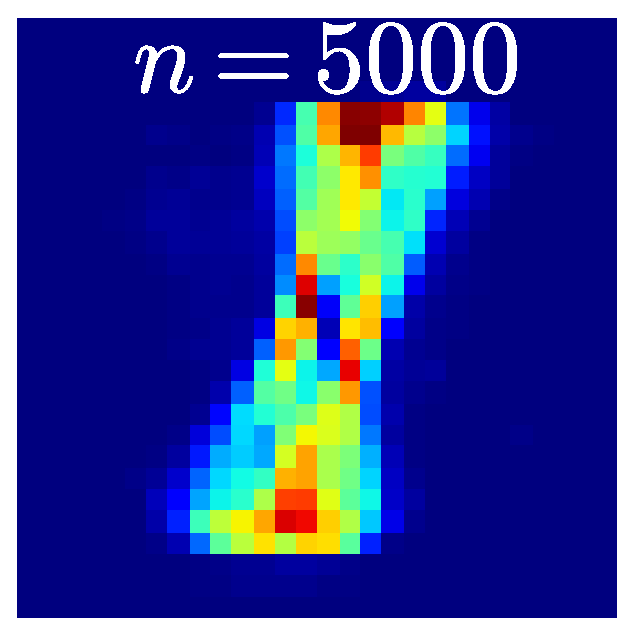
\includegraphics[width=0.1\linewidth]{figures/pixel_relevance_5000.eps}
		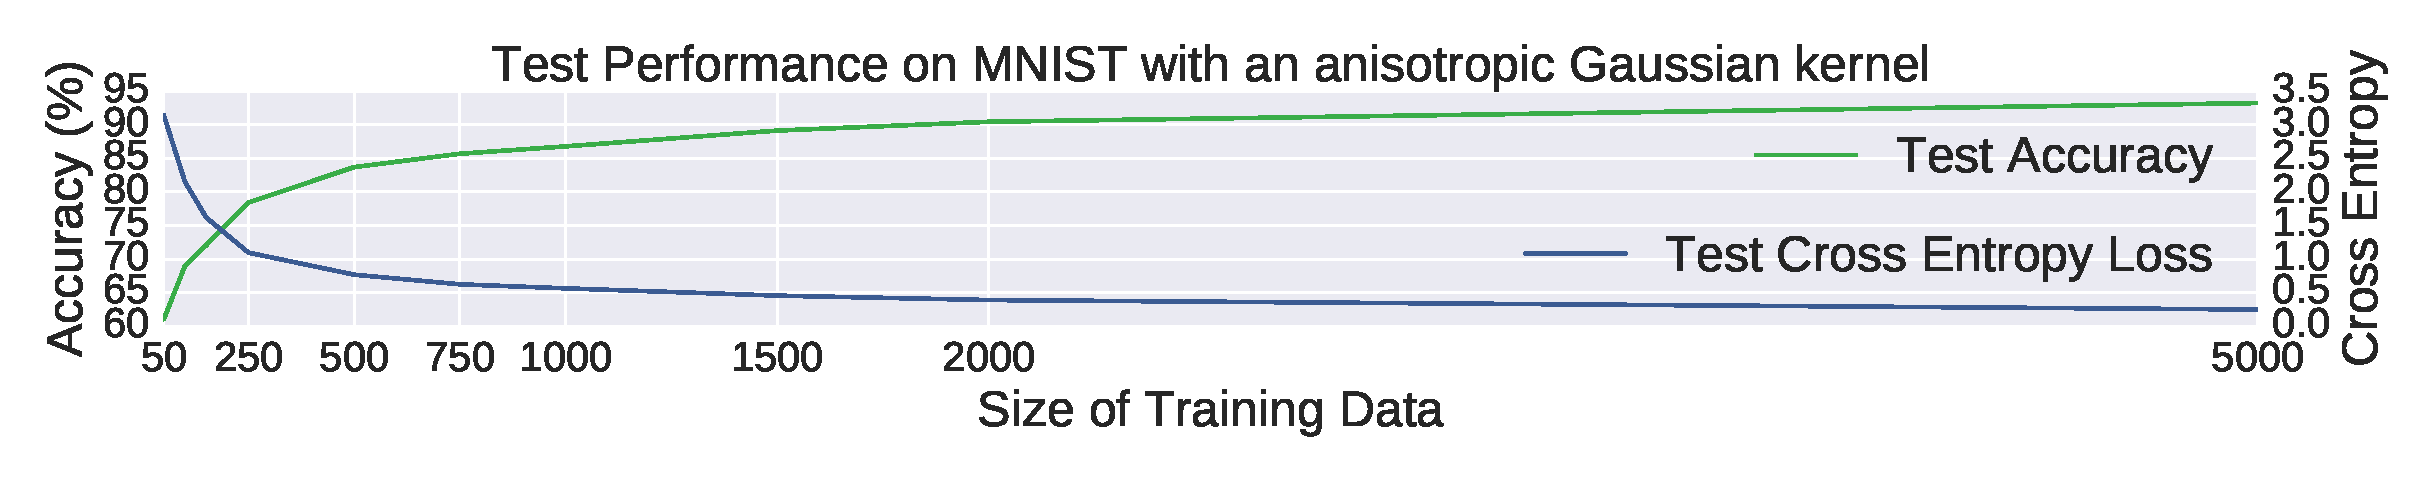
\includegraphics[width=\linewidth]{figures/test_performance.eps}
		\caption{Training the kernel embedding classifier on the MNIST digits dataset with an anisotropic Gaussian kernel. Top: Learned length scales for each pixel; Bottom: Performance on the test set.}
		\label{fig:pixel_relevance}
	\end{figure}
		
	\begin{figure}[t]
		\centering
		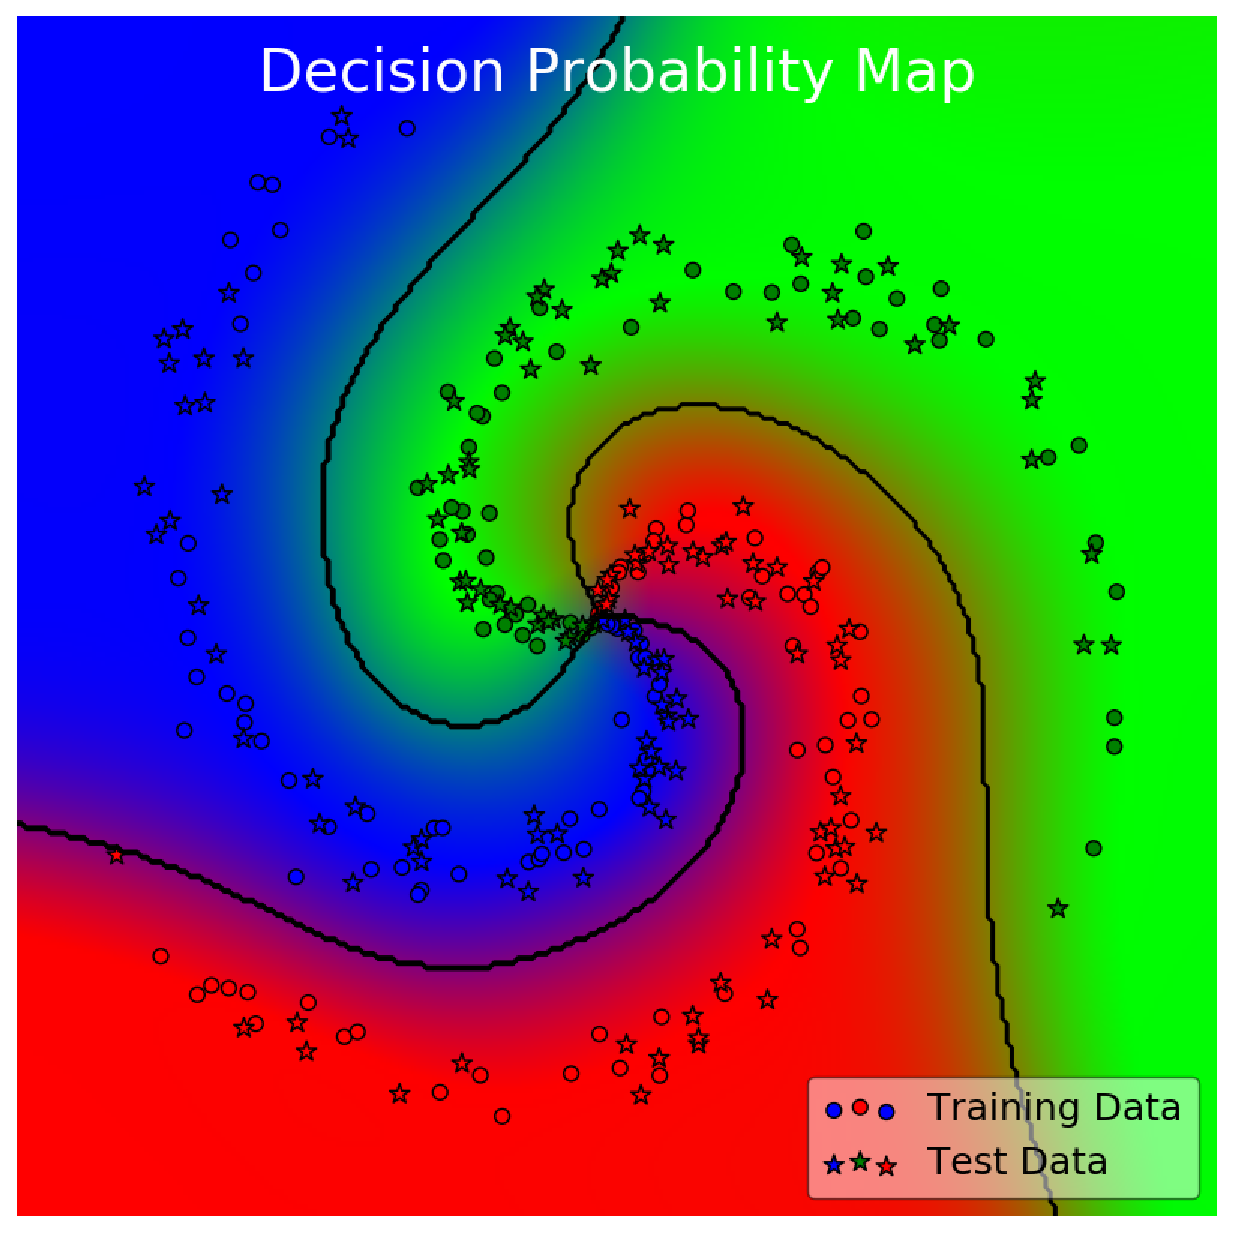
\includegraphics[width=0.25\linewidth]{figures/spiral_all_final.eps}
		\caption{.}
		\label{fig:spiral}
	\end{figure}
	
\section{Conclusion}

	\note{Summarise main contribution.}
	
	Contrary to parametric models, nonlinear kernels produce nonparametric classifiers, and thus its model capacity grows with increasing data. Within a large enough family of kernels $k_{\theta}$, the kernel embedding classifier always has the capacity to shatter the training data and produce zero training error. This is precisely the quality Rademacher complexity measures. Given that it has such capabilities, we instead focus on learning the simplest model, so that it can generalise well to unseen data. By jointly minimising the training risk and the Rademacher complexity bound, we are effectively removing unnecessarily complex models while maintaining good generalisation performance. Without the Rademacher complexity bound $r(\theta, \lambda)$, the classifier can easily overfit by adapting its model capacity to the training data closely. In short, while parametric models have limited capacity and thus trying to learn to perform well on a training set to its best ability is a good indicator to test performance, nonparametric models has infinite capacity and need to learn not to exploit this capacity on training data and instead learn the simplest pattern it can to be able to infer about new test instances.
	
\small
\bibliographystyle{apalike}
\bibliography{kernel_embedding}

\newpage
\appendix

\section{Information Entropy}
\label{app:information_entropy}

	The kernel embedding classifier provides decision probabilities instead of just a single label prediction. Such a probabilistic classifier allows us to quantify the uncertainty of its predictions for any given example $x \in \mathcal{X}$ through the information entropy \citep{shannon1951prediction, jaynes1957information}. This is ideal for detecting the decision boundaries of the classifier and areas of low data density.
	
	We present two main approaches for inferring the information entropy from the classifier. Specifically, we would like to infer estimates for $h(x) := \mathbb{H}[Y | X = x] = - \sum_{c = 1}^{m} p_{c}(x) \log{p_{c}(x)} $, the information entropy of the possible labels $Y$ for a given example $X = x$.
	
	The first approach is straight forward, which involves simply computing the information entropy with the clip normalised probabilities \eqref{eq:empirical_decision_probability_clip_normalised}, at the query point $x \in \mathcal{X}$,
	\begin{equation}
		\tilde{h}(x) := - \sum_{c = 1}^{m} \tilde{p}_{c}(x) \log{\tilde{p}_{c}(x)}.
	\label{eq:entropy_clip_normalise}
	\end{equation}
	We call \eqref{eq:entropy_clip_normalise} the \textit{clip-normalised information entropy}. Since $\tilde{p}_{c}(x)$ converges pointwise to $p_{c}(x)$ with increasing data, $\tilde{h}(x)$ also converges pointwise to $h(x)$.
	
	Just as decision probabilities can be expressed as an expectation of indicator functions, information entropy can be expressed as expected information \footnote{Note that while $\mathbb{P}[Y = c | X = x]$ is a constant, we employ the shorthand notation $\mathbb{P}[Y| X = x]$ for the random variable $g(Y)$ where $g(y) := \mathbb{P}[Y = y | X = x]$.},
	\begin{equation}
	\begin{aligned}
		\mathbb{H}[Y | X = x] &= - \sum_{c = 1}^{m} \mathbb{P}[Y = c| X = x] \log{\mathbb{P}[Y = c | X = x]} \\
		&= \mathbb{E}[- \log{\mathbb{P}[Y | X = x]} | X = x] \\
		&= \mathbb{E}[u_{x}(Y) | X = x],
	\end{aligned}
	\end{equation}
	where $u_{x}(y) := - \log{\mathbb{P}[Y = y | X = x]}$ is the \textit{information} (in nats) we would gain when we discover that example $x$ actually has label $y$. If $u_{x} : \mathbb{N}_{m} \to \mathbb{R}$ is in the RKHS $\mathcal{H}_{\delta}$, then we know that this expectation can also be approximated by $\langle \hat{\mu}_{Y | X = x}, u_{x} \rangle$. This is the basis of our second approach.
	
	Assuming that $\mathbb{P}[Y = y | X = x]$ is never exactly zero for all labels $y \in \mathcal{Y}$ and examples $x \in \mathcal{X}$, then $u_{x}(y)$ is bounded on its discrete domain $\mathbb{N}_{m}$. We can thus write $u_{x} = \sum_{c = 1}^{m} - \log{\mathbb{P}[Y = c | X = x]} \delta(c, \cdot)$ which shows that $u_{x}$ is in the span of the canonical kernel features and is thus in the RKHS. Hence, similar to the case with decision probabilities, with $u_{x} \in \mathcal{H}_{\delta}$ and $\bvec{u}_{x} := \{u_{x}(y_{i})\}_{i = 1}^{n}$ we let $g = u_{x}$ in \eqref{eq:empirical_conditional_expectation} and estimate $h(x)$ by
	\begin{equation}
		\langle \hat{\mu}_{Y | X = x}, u_{x} \rangle = \bvec{u}_{x}^{T} (K + n \lambda I)^{-1} \bvec{k}(x).
	\end{equation}
	Unfortunately, $u_{x}$ is not known exactly, since $\mathbb{P}[Y = y | X = x]$ is not known exactly. Instead, since $\hat{p}_{c}(x)$ is a consistent estimate for $\mathbb{P}[Y = c | X = x]$ by \cref{thm:probability_convergence}, we propose to replace $u_{x}(y)$ with the negative log of $\hat{p}_{y}(x)$. However, we cannot simply take the log of this estimator, as $\hat{p}_{y}(x)$ may produce non-positive estimates to the prediction probabilities. The straight forward way to mitigate this problem is to clip $\hat{p}_{y}(x)$ from the bottom by a very small number, before taking the log. However, experiments show that this produces non-smooth estimates over $\mathcal{X}$ and the degree of smoothness varies drastically between different choices of that small number (see \cref{app:design_choices}). Instead, in virtue of the fact that $\lim_{p \to 0} - p \log{p} = 0$ even though $\lim_{p \to 0} - \log{p} = \infty$, we simply define the information estimate $\hat{u}_{x}(y)$ as zero if the empirical decision probability is non-positive,
	\begin{equation}
		\hat{u}_{x}(y) := \begin{cases}
		- \log{\hat{p}_{y}(x)} & \mathrm{if } \quad \hat{p}_{y}(x) > 0 \\
		0 & \mathrm{otherwise}. \end{cases}
	\label{eq:empirical_information}
	\end{equation}
	It remains to show that $\hat{u}_{x} \in \mathcal{H}_{\delta}$. Indeed, the identity $\hat{u}_{x} = \sum_{c = 1}^{m} \hat{u}_{x}(c) \delta(c, \cdot)$ holds and thus $\hat{u}_{x}$ is in the span of the kernel canonical features. We then arrive at the following estimate for $h(x)$,
	\begin{equation}
		\hat{h}(x) := \langle \hat{\mu}_{Y | X = x}, \hat{u}_{x} \rangle = \hat{\bvec{u}}_{x}^{T} (K + n \lambda I)^{-1} \bvec{k}(x),
		\label{eq:empirical_information_entropy}
	\end{equation}
	where $\hat{\bvec{u}}_{x} := \{\hat{u}_{x}(y_{i})\}_{i = 1}^{n}$. Similar to the case with decision probabilities \eqref{eq:decision_probability}, the information entropy estimate \eqref{eq:empirical_information_entropy} is not guaranteed to be non-negative. However, in practice these negative values are close to zero. Furthermore, negative estimated information entropy implies that the model is very confident about its prediction, and it suffices to simply clip the entropy at zero if strict information entropy is required (see \cref{app:design_choices}). We give the proof of convergence of \eqref{eq:empirical_information_entropy} in \cref{app:convergence_theorems}.
	\begin{theorem}[Uniform Convergence of Empirical Information Entropy Function]
		\label{thm:entropy_convergence_copy}
		Assuming that $k(x, \cdot)$ is in the image of $C_{XX}$, the empirical information entropy function $\hat{h} : \mathcal{X} \to \mathbb{R}$ \eqref{eq:empirical_information_entropy} converges uniformly to the true information entropy function $h : \mathcal{X} \to [0, \infty)$ at a stochastic rate of at least $O_{p}((n \lambda)^{-\frac{1}{2}} + \lambda^{\frac{1}{2}})$.
	\end{theorem}
	
\section{Convergence Theorems}
\label{app:convergence_theorems}

	In this section we provide a few theorems, lemmas, and derivations which proves the convergence properties of estimators derived from our kernel embedding classifier.
	
	We consider the case in which a dataset, represented by the collection of random variables $\{X_{i}, Y_{i}\}_{i = 1}^{n}$ where $X_{i} : \Omega \to \mathcal{X}$,  $Y_{i} : \Omega \to \mathcal{Y}$ for all $i \in \mathbb{N}_{n}$, is collected in a \textit{iid} fashion from some distribution $\mathbb{P}_{X Y}$. That is $\{X_{i}, Y_{i}\} \sim \mathbb{P}_{X Y}$ for all $i \in \mathbb{N}_{n}$ and each observed sample is independent from each other. Suppose we have an estimator function $\hat{f}^{(n)} : \mathcal{X} \to \mathbb{R}$ which is to estimate some target function  $f : \mathcal{X} \to \mathbb{R}$, usually but not necessarily derived from $\mathbb{P}_{Y |X }$, empirically using the collected dataset $\{X_{i}, Y_{i}\}_{i = 1}^{n}$ of size $n \in \mathbb{N}_{+}$. Here, we use the superscript $(n)$ to denote the estimator's dependence on the dataset. From this point on, we drop this superscript to avoid cluttered notation. However, one should keep in mind that $\hat{f}$ is estimated using the dataset $\{X_{i}, Y_{i}\}_{i = 1}^{n}$ and is thus random over the possible data observation events $\omega \in \Omega$. We would like to provide a sense of the stochastic convergence of $\hat{f}$ to $f$ by providing an upper bound of their absolute pointwise difference $| \hat{f}(x) - f(x) |$ which we know convergences to zero at some stochastic rate. Since the kernel embedding classifier is based on conditional embeddings, this upper bound will be provided by the RKHS norm of the error between empirical and true conditional embeddings. Specifically, the empirical conditional embedding stochastically converges to the true conditional embedding $\mu_{Y | X = x}$ in the RKHS norm at a rate of $O_{p}((n \lambda)^{-\frac{1}{2}} + \lambda^{\frac{1}{2}})$, under the assumption that $k(x, \cdot)$ is in the image of $C_{XX}$ \cite[Theorem 6]{song2009hilbert}. That is,
	
		\begin{equation}
			\forall x \in \mathcal{X}, \; \epsilon > 0, \; \exists M_{\epsilon} > 0 \quad s.t. \quad \mathbb{P}\Big[\big\| \hat{\mu}_{Y | X = x} - \mu_{Y | X = x} \big\|_{\mathcal{H}_{l}} > M_{\epsilon} \Big((n \lambda)^{-\frac{1}{2}} + \lambda^{\frac{1}{2}}\Big)\Big] < \epsilon.
		\label{eq:empirical_conditional_embedding_stochastic_convergence}
		\end{equation}
	
	\begin{theorem}[Pointwise and Uniform Convergence of Estimators based on Conditional Embeddings]
		\label{thm:pointwise_uniform_convergence}
		Suppose that $k(x, \cdot)$ is in the image of $C_{XX}$ and that there exists $0 \leq \gamma(x) < \infty$ such that for some estimator function $\hat{f} : \mathcal{X} \to \mathbb{R}$ and target function  $f : \mathcal{X} \to \mathbb{R}$,
		
		\begin{equation}
			| \hat{f}(x) - f(x) | \leq \gamma(x) \big\| \hat{\mu}_{Y | X = x} - \mu_{Y | X = x} \big\|_{\mathcal{H}_{l}}, \forall x \in \mathcal{X},
		\label{eq:estimator_error_bound}
		\end{equation}
		 
		then the estimator $\hat{f}$ converges pointwise to the target $f$ at a stochastic rate of at least $O_{p}((n \lambda)^{-\frac{1}{2}} + \lambda^{\frac{1}{2}})$. Further, if $\gamma(x) = \gamma$ is independent of $x \in \mathcal{X}$, then this convergence is uniform.
		
		\begin{proof}
			
			Suppose that there exists $0 \leq \gamma(x) < \infty$ such that \eqref{eq:estimator_error_bound} is satisfied. Note that this statement holds for all possible datasets represented by the collection of random variables $\{X_{i}, Y_{i}\}_{i = 1}^{n}$ where $X_{i} : \Omega \to \mathcal{X}$,  $Y_{i} : \Omega \to \mathcal{Y}$ for all $i \in \mathbb{N}_{n}$. Thus, for any constant $C$, the implication statement $\big\| \hat{\mu}_{Y | X = x} - \mu_{Y | X = x} \big\|_{\mathcal{H}_{\delta}} \leq C \implies | \hat{f}(x) - f(x) | \leq C \gamma(x)$ holds for all possible data observation events $\omega \in \Omega$. Writing this explicitly in event space translates this to a probability statement,
			
			\begin{equation}
			\begin{aligned}
				\{\omega \in \Omega : \big\| \hat{\mu}_{Y | X = x} - \mu_{Y | X = x} \big\|_{\mathcal{H}_{l}} \leq C\} &\subseteq \{\omega \in \Omega : | \hat{f}(x) - f(x) | \leq C \gamma(x)\} \\
				\implies \mathbb{P}\Big[\big\| \hat{\mu}_{Y | X = x} - \mu_{Y | X = x} \big\|_{\mathcal{H}_{l}} \leq C\Big] &\leq \mathbb{P}\Big[| \hat{f}(x) - f(x) | \leq C \gamma(x) \Big].
			\label{eq:probability_statement}
			\end{aligned}
			\end{equation}
			
			Since we assume that $k(x, \cdot) \in \mathrm{image}(C_{XX})$, statement \eqref{eq:empirical_conditional_embedding_stochastic_convergence} is valid. By letting $C = M_{\epsilon} ((n \lambda)^{-\frac{1}{2}} + \lambda^{\frac{1}{2}})$ in \eqref{eq:probability_statement}, we immediately have that the probability inequality in statement \eqref{eq:empirical_conditional_embedding_stochastic_convergence} is also true if we replace $\| \hat{\mu}_{Y | X = x} - \mu_{Y | X = x} \|$ with $| \hat{f}(x) - f(x) |$ and $M_{\epsilon}$ with $\gamma(x) M_{\epsilon}$,
			
			\begin{equation}
			\begin{aligned}
			\mathbb{P}\Big[\big\| \hat{\mu}_{Y | X = x} - \mu_{Y | X = x} \big\|_{\mathcal{H}_{l}} > M_{\epsilon} \Big((n \lambda)^{-\frac{1}{2}} + \lambda^{\frac{1}{2}}\Big)\Big] &< \epsilon \\
			\implies 1 - \mathbb{P}\Big[\big\| \hat{\mu}_{Y | X = x} - \mu_{Y | X = x} \big\|_{\mathcal{H}_{l}} \leq M_{\epsilon} \Big((n \lambda)^{-\frac{1}{2}} + \lambda^{\frac{1}{2}}\Big)\Big] &< \epsilon \\
			\implies \mathbb{P}\Big[\big\| \hat{\mu}_{Y | X = x} - \mu_{Y | X = x} \big\|_{\mathcal{H}_{l}} \leq M_{\epsilon} \Big((n \lambda)^{-\frac{1}{2}} + \lambda^{\frac{1}{2}}\Big)\Big] &> 1 -  \epsilon \\
			\implies \mathbb{P}\Big[| \hat{f}(x) - f(x) | \leq \gamma(x) M_{\epsilon} \Big((n \lambda)^{-\frac{1}{2}} + \lambda^{\frac{1}{2}}\Big)\Big] &> 1 -  \epsilon \\
			\implies 1 - \mathbb{P}\Big[| \hat{f}(x) - f(x) | \leq \gamma(x) M_{\epsilon} \Big((n \lambda)^{-\frac{1}{2}} + \lambda^{\frac{1}{2}}\Big)\Big] &< \epsilon \\
			\implies \mathbb{P}\Big[| \hat{f}(x) - f(x) | > \gamma(x) M_{\epsilon} \Big((n \lambda)^{-\frac{1}{2}} + \lambda^{\frac{1}{2}}\Big)\Big] &< \epsilon.
			\end{aligned}	
			\end{equation}
			
			where we employed statement \eqref{eq:probability_statement} between the third and fourth line for $C = M_{\epsilon} ((n \lambda)^{-\frac{1}{2}} + \lambda^{\frac{1}{2}})$. Therefore, since $M_{\epsilon}$ is arbitrary, define $\tilde{M}_{\epsilon}(x) := \gamma(x) M_{\epsilon}$ so that, with the above result, the statement \eqref{eq:empirical_conditional_embedding_stochastic_convergence} implies the following,

			\begin{equation}
				\forall x \in \mathcal{X}, \; \epsilon > 0, \; \exists \tilde{M}_{\epsilon}(x) > 0 \quad s.t. \quad \mathbb{P}\Big[\big| \hat{f}(x) - f(x) \big| > \tilde{M}_{\epsilon}(x) \Big((n \lambda)^{-\frac{1}{2}} + \lambda^{\frac{1}{2}}\Big)\Big] < \epsilon.
			\end{equation}
	
			In other words, the function $\hat{f}$ stochastically converges pointwise to $f$ with a rate of at least $O_{p}((n \lambda)^{-\frac{1}{2}} + \lambda^{\frac{1}{2}})$. The convergence is pointwise as the constant $\tilde{M}_{\epsilon}(x)$ may be different for each point $x \in \mathcal{X}$. If $\gamma(x) = \gamma$ such that $\tilde{M}_{\epsilon}(x) = \tilde{M}_{\epsilon}$ does not depend on $x \in \mathcal{X}$, then this stochastic convergence is uniform in its domain $\mathcal{X}$.
		\end{proof}
		
	\end{theorem}
	
	With \cref{thm:pointwise_uniform_convergence}, we can now show the convergence of various estimators based on the conditional embedding, as long as we can show that their estimator error is upper bounded by a multiple of the conditional embedding error in the RKHS norm. As such, we turn to the convergence of the empirical decision probability function \eqref{eq:empirical_decision_probability} below.

	\begin{theorem}[Uniform Convergence of Empirical Decision Probability Function]
		\label{thm:probability_convergence}
		Assuming that $k(x, \cdot)$ is in the image of $C_{XX}$, the empirical decision probability function $\hat{p}_{c} : \mathcal{X} \to \mathbb{R}$ \eqref{eq:empirical_decision_probability} converges uniformly to the true decision probability $p_{c} : \mathcal{X} \to [0, 1]$ \eqref{eq:decision_probability} at a stochastic rate of at least $O_{p}((n \lambda)^{-\frac{1}{2}} + \lambda^{\frac{1}{2}})$ for all $c \in \mathcal{Y} = \mathbb{N}_{m}$.
		
		\begin{proof}
			Consider the pointwise absolute difference between the decision probability and its empirical estimate,
			
			\begin{equation}
			\begin{aligned}
				| \hat{p}_{c}(x) - p_{c}(x) | &= | \langle \hat{\mu}_{Y | X = x}, \mathbb{1}_{c} \rangle - \langle \mu_{Y | X = x}, \mathbb{1}_{c} \rangle | \\
				&= | \langle \hat{\mu}_{Y | X = x} - \mu_{Y | X = x}, \mathbb{1}_{c} \rangle | \\
				&\leq \big\| \hat{\mu}_{Y | X = x} - \mu_{Y | X = x} \big\|_{\mathcal{H}_{\delta}} \big\| \mathbb{1}_{c} \big\|_{\mathcal{H}_{\delta}},
			\label{eq:decision_probability_error_upper_bound}
			\end{aligned}
			\end{equation}
			
			where the last inequality follows from the Cauchy–Schwarz inequality in a Hilbert space.
			
			From \eqref{eq:indicator_function}, since $\mathbb{1}_{c} = \delta(c, \cdot)$ and using the fact that $\delta$ is a reproducing kernel, we have that for all $c \in \mathcal{Y} = \mathbb{N}_{m}$.
			
			\begin{equation}
			\begin{aligned}
				\big\| \mathbb{1}_{c} \big\|_{\mathcal{H}_{\delta}}^{2} = \langle \mathbb{1}_{c}, \mathbb{1}_{c} \rangle = \langle \delta(c, \cdot), \delta(c, \cdot) \rangle = \delta(c, c) = 1.
			\label{eq:indicator_rkhs_norm}
			\end{aligned}
			\end{equation}
			
			Therefore, by \cref{thm:pointwise_uniform_convergence} with $\gamma(x) = 1$ independent of $x \in \mathcal{X}$, $\hat{p}_{c}$ converges uniformly to $p_{c}$ at a stochastic rate of at least $O_{p}((n \lambda)^{-\frac{1}{2}} + \lambda^{\frac{1}{2}})$ for all $c \in \mathcal{Y} = \mathbb{N}_{m}$.
			
			%		Consequently, $| \hat{p}_{c}(x) - p_{c}(x) | \leq \big\| \hat{\mu}_{Y | X = x}^{(n)} - \mu_{Y | X = x} \big\|_{\mathcal{H}_{\delta}}$ for all $x \in \mathcal{X}$, where the right hand side of which approaches zero stochastically at rate $O_{p}((n \lambda)^{-\frac{1}{2}} + \lambda^{\frac{1}{2}})$ since we assume that $k(x, \cdot) \in \mathrm{image}(C_{XX})$, so that $\hat{p}_{c}$ converges pointwise to $p_{c}$ at least at this rate. The convergence rate does not depend on $x \in \mathcal{X}$, so this (stochastic) convergence is pointwise uniform.
			
%			Consequently, for all $x \in \mathcal{X}$ and $c \in \mathcal{Y}$, we have 
%			
%			\begin{equation}
%				| \hat{p}_{c}(x) - p_{c}(x) | \leq \big\| \hat{\mu}_{Y | X = x} - \mu_{Y | X = x} \big\|_{\mathcal{H}_{\delta}}.
%			\label{eq:uniform_convergence}
%			\end{equation}
%			
%			This is true for all possible datasets represented by the collection of random variables $\{X_{i}, Y_{i}\}_{i = 1}^{n}$ where $X_{i} : \Omega \to \mathcal{X}$,  $Y_{i} : \Omega \to \mathcal{Y}$ for all $i \in \mathbb{N}_{n}$. Thus, for any constant $C$, the implication statement $\big\| \hat{\mu}_{Y | X = x} - \mu_{Y | X = x} \big\|_{\mathcal{H}_{\delta}} \leq C \implies | \hat{p}_{c}(x) - p_{c}(x) | \leq C$ holds for all possible data observation events $\omega \in \Omega$. Writing this explicitly in event space translates this to a probability statement,
%			
%			\begin{equation}
%			\begin{aligned}
%			\{\omega \in \Omega : \big\| \hat{\mu}_{Y | X = x} - \mu_{Y | X = x} \big\|_{\mathcal{H}_{\delta}} \leq C\} &\subseteq \{\omega \in \Omega : | \hat{p}_{c}(x) - p_{c}(x) | \leq C\} \\
%			\implies \mathbb{P}\Big[\big\| \hat{\mu}_{Y | X = x} - \mu_{Y | X = x} \big\|_{\mathcal{H}_{\delta}} \leq C\Big] &\leq \mathbb{P}\Big[| \hat{p}_{c}(x) - p_{c}(x) | \leq C \Big].
%			\label{eq:probability_statement}
%			\end{aligned}
%			\end{equation}
%			
%			Since we assume that $k(x, \cdot) \in \mathrm{image}(C_{XX})$, statement \eqref{eq:empirical_conditional_embedding_stochastic_convergence} is valid. By letting $C = M_{\epsilon} ((n \lambda)^{-\frac{1}{2}} + \lambda^{\frac{1}{2}})$ in \eqref{eq:probability_statement}, we immediately have that the probability inequality in statement \eqref{eq:probability_statement} is also true if we replace $\| \hat{\mu}_{Y | X = x} - \mu_{Y | X = x} \|$ with $| \hat{p}_{c}(x) - p_{c}(x) |$, % the RKHS norm between the empirical and true embeddings to the absolute difference between the empirical decision probability and the true decision probability,
%			
%			\begin{equation}
%			\begin{aligned}
%			\mathbb{P}\Big[\big\| \hat{\mu}_{Y | X = x} - \mu_{Y | X = x} \big\|_{\mathcal{H}_{l}} > M_{\epsilon} \Big((n \lambda)^{-\frac{1}{2}} + \lambda^{\frac{1}{2}}\Big)\Big] &< \epsilon \\
%			\implies 1 - \mathbb{P}\Big[\big\| \hat{\mu}_{Y | X = x} - \mu_{Y | X = x} \big\|_{\mathcal{H}_{l}} \leq M_{\epsilon} \Big((n \lambda)^{-\frac{1}{2}} + \lambda^{\frac{1}{2}}\Big)\Big] &< \epsilon \\
%			\implies \mathbb{P}\Big[\big\| \hat{\mu}_{Y | X = x} - \mu_{Y | X = x} \big\|_{\mathcal{H}_{l}} \leq M_{\epsilon} \Big((n \lambda)^{-\frac{1}{2}} + \lambda^{\frac{1}{2}}\Big)\Big] &> 1 -  \epsilon \\
%			\implies \mathbb{P}\Big[| \hat{p}_{c}(x) - p_{c}(x) | \leq M_{\epsilon} \Big((n \lambda)^{-\frac{1}{2}} + \lambda^{\frac{1}{2}}\Big)\Big] &> 1 -  \epsilon \\
%			\implies 1 - \mathbb{P}\Big[| \hat{p}_{c}(x) - p_{c}(x) | \leq M_{\epsilon} \Big((n \lambda)^{-\frac{1}{2}} + \lambda^{\frac{1}{2}}\Big)\Big] &< \epsilon \\
%			\implies \mathbb{P}\Big[| \hat{p}_{c}(x) - p_{c}(x) | > M_{\epsilon} \Big((n \lambda)^{-\frac{1}{2}} + \lambda^{\frac{1}{2}}\Big)\Big] &< \epsilon.
%			\end{aligned}	
%			\end{equation}
%			
%			In other words, the function $\hat{p}_{c}$ stochastically converges pointwise to $p_{c} := \mathbb{P}[Y = c | X = \cdot]$ with a rate of at least $O_{p}((n \lambda)^{-\frac{1}{2}} + \lambda^{\frac{1}{2}})$. The convergence rate does not depend on $x \in \mathcal{X}$ nor $c \in \mathbb{N}_{m}$, so this stochastic convergence is pointwise uniform in its domain $\mathcal{X}$ across all label classes.
			
		\end{proof}
	\end{theorem}
	
	The above proof is for uniform convergence over all $x \in \mathcal{X}$ at the stochastic rate of at least $O_{p}((n \lambda)^{-\frac{1}{2}} + \lambda^{\frac{1}{2}})$. Intuitively, however, for stationary zero-centred kernels like the Gaussian kernel, the convergence rate may be higher at regions of high data density, since the kernel effects, being centred around the training data, are stronger at these regions. The worse case convergence rate described here in the theorem would be a tight lower bound for regions in $\mathcal{X}$ with lower data density, where the kernel effects have decayed and most empirical probabilities are smaller and further from summing up to one.
	
	Because the label space $\mathcal{Y} = \mathbb{N}_{m}$ is discrete and finite, \textit{bounded} functions $g \in \mathcal{H}_{\delta}$ in the RKHS are actually equivalent to their vector representations $\bvec{g} := \{g(c)\}_{c = 1}^{m}$, because one can always write $g = \sum_{c = 1}^{m} g(c) \delta(c, \cdot)$. This immediately implies that inner products in this space are simply the usual dot products in a Euclidean space, since
	
	\begin{equation}
	\begin{aligned}
	\langle g_{1}, g_{2} \rangle_{\mathcal{H}_{\delta}} &= \bigg\langle \sum_{c = 1}^{m} g_{1}(c) \delta(c, \cdot), \sum_{c' = 1}^{m} g_{2}(c') \delta(c', \cdot)  \bigg\rangle_{\mathcal{H}_{\delta}} \\
	&= \sum_{c = 1}^{m} \sum_{c' = 1}^{m} g_{1}(c) g_{2}(c') \langle \delta(c, \cdot), \delta(c', \cdot) \rangle_{\mathcal{H}_{\delta}} \\
	&= \sum_{c = 1}^{m} g_{1}(c) g_{2}(c) \\
	&= \bvec{g}_{1} \cdot \bvec{g}_{2}.
	\end{aligned}
	\end{equation}
	
	Consequently, the RKHS norm for bounded functions $g \in \mathcal{H}_{\delta}$ is simply the $\ell_{2}$-norm of its vector representation $\bvec{g}$,
	
	\begin{equation}
	\lVert g \rVert_{\mathcal{H}_{\delta}} = \lVert \bvec{g} \rVert_{\ell_{2}}.
	\label{eq:rkhs_norm_is_l2_norm}
	\end{equation}

	A special and convenient result that arises due to this discrete and finite label space is that the decision probabilities and its empirical estimate are simply the conditional embeddings and its empirical estimate.
	
	\begin{claim}[Decision Probabilities are Conditional Embeddings]
	\label{thm:probability_is_embedding}
	
		The decision probability for class $c \in \mathbb{N}_{m}$ given an example $x \in \mathcal{X}$ is the conditional embedding with $l = \delta$ conditioned at example $x$ evaluated at label $c$,
			
		\begin{equation}
			p_{c}(x) := \mathbb{P}[Y = c | X = x] = \mu_{Y | X = x}(c).
		\end{equation}
		
		
		\begin{proof} Since indicator functions are the canonical features of the label RKHS $\mathcal{H}_{\delta}$, we employ the fact that expectations of indicator functions are probabilities to prove this claim,
			
			\begin{equation}
			\begin{aligned}
				\mu_{Y | X = x}(c) :=& \mathbb{E}[l(Y, c) | X = x ]= \mathbb{E}[\delta(Y, c) | X = x] \\
				=& \mathbb{E}[\mathbb{1}_{c}(Y) | X = x] = \mathbb{P}[Y \in \{c\} | X = x] \\
				=& \mathbb{P}[Y = c | X = x] := p_{c}(x).
			\end{aligned}
			\end{equation}
		\end{proof}

	\end{claim}
	
	\begin{claim}[Empirical Decision Probabilities are Empirical Conditional Embeddings]
	\label{thm:empirical_probability_is_embedding}
	
		The empirical decision probability \eqref{eq:empirical_decision_probability} for class $c \in \mathbb{N}_{m}$ given an example $x \in \mathcal{X}$ is the empirical conditional embedding with $l = \delta$ conditioned at example $x$ evaluated at label $c$,
			
		\begin{equation}
			\hat{p}_{c}(x) = \hat{\mu}_{Y | X = x}(c).
		\end{equation}
		
		Therefore, $\hat{\bvec{p}}(x) \equiv \hat{\mu}_{Y | X = x}$.
				
		\begin{proof}
			
			Let the canonical feature maps of $\mathcal{X}$ and $\mathcal{Y}$ be $\phi(x) = k(x, \cdot)$ and $\psi(y) = l(y, \cdot) = \delta(y, \cdot)$, then the empirical conditional embedding is defined by
			
			\begin{equation}
				\hat{\mu}_{Y | X = x} := \hat{\mathcal{U}}_{Y | X} \phi(x)
			\end{equation}
			
			By the reproducing property, the evaluation of $\hat{\mu}_{Y | X = x} \in \mathcal{H}_{l}$ is given by a dot product,
	
			\begin{equation}
			\begin{aligned}
				\hat{\mu}_{Y | X = x}(c) &= \langle l(c, \cdot), \hat{\mu}_{Y | X = x} \rangle \\
				&= \langle \psi(c), \hat{\mu}_{Y | X = x} \rangle \\
				&= \psi(c)^{T} \hat{\mu}_{Y | X = x} \\
				&= \psi(c)^{T} \hat{\mathcal{U}}_{Y | X} \phi(x) \\
				&= \psi(c)^{T} \Psi (K + n \lambda I)^{-1} \Phi^{T} \phi(x) \\
				&= \bvec{l}_{c}^{T} (K + n \lambda I)^{-1} \bvec{k}(x), \\
			\end{aligned}
			\end{equation}
			
			where $\bvec{l}_{c} := \{l(y_{i}, c)\}_{i = 1}^{n}$ and $\bvec{k}_{x} := \{k(x_{i}, x)\}_{i = 1}^{n}$. While the notation $\bvec{l}_{c}$ is usually avoided due do its similarity to $\bvec{1}_{c}$, in this context they happen to represent equal quantities,
			
			\begin{equation}
				\bvec{l}_{c} := \{l(y_{i}, c)\}_{i = 1}^{n} = \{\delta(y_{i}, c)\}_{i = 1}^{n} = \{\mathbb{1}_{c}(y_{i})\}_{i = 1}^{n} =: \bvec{1}_{c}.
			\end{equation}
			
			The claim then immediately follows by the definition of our decision probability estimator,
			
			\begin{equation}
				\hat{\mu}_{Y | X = x}(c) = \bvec{1}_{c}^{T} (K + n \lambda I)^{-1} \bvec{k}(x) =: \hat{p}_{c}(x).
			\end{equation}
		\end{proof}
		
	\end{claim}
	
	Since we have identified the equivalence of decision probabilities and the conditional embedding, we can now also show that the empirical decision probability vector also converges to the true decision probability vector.

	\begin{lemma}[Uniform Convergence of Empirical Decision Probability Vector Function in $\ell_{1}$ and $\ell_{2}$]
	\label{thm:probability_vector_convergence} 
	
		Assuming that $k(x, \cdot)$ is in the image of $C_{XX}$, the empirical decision probability vector function $\hat{\bvec{p}} : \mathcal{X} \to \mathbb{R}^{m}$ \eqref{eq:empirical_decision_probability_vector} converges uniformly to the true decision probability vector function $\bvec{p} : \mathcal{X} \to [0, 1]^{m}$ in the $\ell_{2}$-norm, where $\bvec{p}(x) := \{p_{c}(x)\}_{c = 1}^{m}$, at a stochastic rate of at least $O_{p}((n \lambda)^{-\frac{1}{2}} + \lambda^{\frac{1}{2}})$ for all $c \in \mathcal{Y} = \mathbb{N}_{m}$.
		
		\begin{proof}
			For convergence in $\ell_{1}$, we simply extend \cref{thm:probability_convergence}, which proved that each entry of $\hat{\bvec{p}}(x)$ converges pointwise uniformly at a rate of $O_{p}((n \lambda)^{-\frac{1}{2}} + \lambda^{\frac{1}{2}})$ to the corresponding entry of $\bvec{p}(x)$. Since each entry converges stochastically at a rate of $O_{p}((n \lambda)^{-\frac{1}{2}} + \lambda^{\frac{1}{2}})$, then so does the entire vector. More formally, from \eqref{eq:decision_probability_error_upper_bound} and \eqref{eq:indicator_rkhs_norm}, the $\ell_{1}$-norm of the difference can be bounded,
			
			\begin{equation}
			\begin{aligned}
				{\lVert \hat{\bvec{p}}(x) - \bvec{p}(x) \rVert}_{\ell_{1}} :=& \sum_{c = 1}^{m} | \hat{p}_{c}(x) - p_{c}(x) | \\
				\leq& \sum_{c = 1}^{m} \big\| \hat{\mu}_{Y | X = x} - \mu_{Y | X = x} \big\|_{\mathcal{H}_{\delta}} \\
				=& m \big\| \hat{\mu}_{Y | X = x} - \mu_{Y | X = x} \big\|_{\mathcal{H}_{\delta}}
			\end{aligned}
			\end{equation}
			
			Therefore, by \cref{thm:pointwise_uniform_convergence} with $\gamma(x) = m$ independent of $x \in \mathcal{X}$, we have uniform convergence in $\ell_{1}$ where we replace all instances of $| \hat{f}(x) - f(x) |$ in the proof of \cref{thm:pointwise_uniform_convergence} with ${\lVert \hat{\bvec{p}}(x) - \bvec{p}(x) \rVert}_{\ell_{1}}$.
			
			For convergence in $\ell_{2}$, we show that the $\ell_{2}$-norm of the difference between the true and empirical decision probability vector functions is the same as the RKHS norm of the difference between the true and empirical conditional embedding, which converges to zero at a stochastic rate of at least $O_{p}((n \lambda)^{-\frac{1}{2}} + \lambda^{\frac{1}{2}})$ for all $x \in \mathcal{X}$ and $c \in \mathcal{Y} = \mathbb{N}_{m}$ \citep{song2009hilbert}. To this end, we use \cref{thm:probability_is_embedding} and \cref{thm:empirical_probability_is_embedding} and write 
			
			\begin{equation}
			\begin{aligned}
				{\lVert \hat{\bvec{p}}(x)  - \bvec{p}(x) \rVert}_{\ell_{2}} &= {\lVert \{ \hat{p}_{c}(x) \}_{c = 1}^{m} - \{ p_{c}(x) \}_{c = 1}^{m} \rVert}_{\ell_{2}} \\
				&= {\lVert \{ \hat{p}_{c}(x) - p_{c}(x) \}_{c = 1}^{m} \rVert}_{\ell_{2}} \\
				&= {\lVert \{ \hat{\mu}_{Y | X = x}(c) - \mu_{Y | X = x}(c)\}_{c = 1}^{m} \rVert}_{\ell_{2}} \\
				&= \| \hat{\bm{\mu}}_{Y | X = x} - \bm{\mu}_{Y | X = x}  \|_{\ell_{2}} \\
				&= {\lVert \hat{\mu}_{Y | X = x} - \mu_{Y | X = x}\rVert}_{\mathcal{H}_{\delta}},
			\end{aligned}
			\end{equation}
			
			where the last equality comes from \eqref{eq:rkhs_norm_is_l2_norm} and the fact that the empirical and true conditional embeddings are bounded functions in the RKHS. Again, by \cref{thm:pointwise_uniform_convergence} with $\gamma(x) = 1$ independent of $x \in \mathcal{X}$, we have uniform convergence in $\ell_{2}$.
		\end{proof}
	\end{lemma}
		
	In \cref{app:information_entropy}, we proposed an estimator for the information entropy $h(x)$ for a prediction at $x \in \mathcal{X}$. Since this estimator is now based on the inner product between the empirical conditional embedding and another empirically estimate function, instead of between the empirical conditional embedding and a known function, it is not immediately clear that such an estimator converges. Nevertheless, intuition tells us that the inner product between two converging quantities should converge. We proceed to show that this intuition is correct.
	
	\begin{theorem}[Convergence of Empirical Information Entropy Function]
		\label{thm:entropy_convergence}
		Assuming that $k(x, \cdot)$ is in the image of $C_{XX}$, the empirical information entropy function $\hat{h} : \mathcal{X} \to \mathbb{R}$ \eqref{eq:empirical_information_entropy} converges pointwise to the true information entropy function $h : \mathcal{X} \to [0, \infty)$ at a stochastic rate of at least $O_{p}((n \lambda)^{-\frac{1}{2}} + \lambda^{\frac{1}{2}})$.
		
		\begin{proof}
			Since we are interested in the asymptotic properties of our estimators when $n \to \infty$, and we have proved that the empirical decision probabilities converges to the true probabilities (\cref{thm:probability_convergence}), the condition $\hat{p}_{c}(x) > 0$ holds for large $n$ such that we simply have $\hat{u}_{x}(c) = - \log{\hat{p}_{c}(x)}$. That is, the effects of clipping for the information estimate \eqref{eq:empirical_information} vanishes.
			
			Consider the pointwise absolute difference between the empirical and true information entropy,
			
			\begin{equation}
			\begin{aligned}
				| \hat{h}(x) - h(x) | &= | \langle \hat{\mu}_{Y | X = x}, \hat{u}_{x} \rangle_{\mathcal{H}_{\delta}} - \langle \mu_{Y | X = x}, u_{x} \rangle_{\mathcal{H}_{\delta}} | \\
				&= | \langle \hat{\mu}_{Y | X = x}, \hat{u}_{x} \rangle_{\mathcal{H}_{\delta}} - \langle \hat{\mu}_{Y | X = x}, u_{x} \rangle_{\mathcal{H}_{\delta}} + \langle \hat{\mu}_{Y | X = x}, u_{x} \rangle_{\mathcal{H}_{\delta}} - \langle \mu_{Y | X = x}, u_{x} \rangle_{\mathcal{H}_{\delta}} | \\
				&\leq | \langle \hat{\mu}_{Y | X = x}, \hat{u}_{x} \rangle_{\mathcal{H}_{\delta}} - \langle \hat{\mu}_{Y | X = x}, u_{x} \rangle_{\mathcal{H}_{\delta}} | + | \langle \hat{\mu}_{Y | X = x}, u_{x} \rangle_{\mathcal{H}_{\delta}} - \langle \mu_{Y | X = x}, u_{x} \rangle_{\mathcal{H}_{\delta}} | \\
				&= | \langle \hat{\mu}_{Y | X = x}, \hat{u}_{x} - u_{x} \rangle_{\mathcal{H}_{\delta}} | + | \langle \hat{\mu}_{Y | X = x} - \mu_{Y | X = x}, u_{x} \rangle_{\mathcal{H}_{\delta}} | \\
				&\leq \| \hat{\mu}_{Y | X = x} \|_{\mathcal{H}_{\delta}} \| \hat{u}_{x} - u_{x} \|_{\mathcal{H}_{\delta}} + \| \hat{\mu}_{Y | X = x} - \mu_{Y | X = x} \|_{\mathcal{H}_{\delta}} \| u_{x} \|_{\mathcal{H}_{\delta}},
			\label{eq:information_entropy_bound}
			\end{aligned}
			\end{equation}
			
			where the we used the triangle inequality and Cauchy–Schwarz inequality in a Hilbert space respectively.
			
			Now, since $l = \delta$ is bounded, so is $\hat{\mu}_{Y | X = x}(c) = \sum_{i = 1}^{n} w_{i} \delta(y_{i}, c)$ for some embedding weights $w_{i}$ and all $c \in \mathbb{N}_{m}$, and thus its RKHS norm is finite for all $n \in \mathbb{N}_{n}$. Similarly, assuming that $p_{c}(x)$ is never exactly zero, $u_{x}(c)$ is also finite for all $c \in \mathbb{N}_{m}$ and thus so is its RKHS norm. We already know that $\| \hat{\mu}_{Y | X = x} - \mu_{Y | X = x} \|_{\mathcal{H}_{\delta}}$ stochastically converges to zero at the rate $O_{p}((n \lambda)^{-\frac{1}{2}} + \lambda^{\frac{1}{2}})$ \citep[Theorem 6]{song2009hilbert}. Thus, it remains to bound $\| \hat{u}_{x} - u_{x} \|_{\mathcal{H}_{\delta}}$ by a multiple of $\| \hat{\mu}_{Y | X = x} - \mu_{Y | X = x} \|_{\mathcal{H}_{\delta}}$.
			
			To this end, we first use \cref{thm:probability_is_embedding} and \cref{thm:empirical_probability_is_embedding} and to express the theoretical and empirical information as the negative log of the embedding, so that it is explicitly written as a function of $c \in \mathcal{Y}$ in $\mathcal{H}_{\delta}$ indexed by $x \in \mathcal{X}$,
			
			\begin{equation}
			\begin{aligned}
				u_{x}(c) &= - \log{p_{c}(x)} = -\log{\mu_{Y | X = x}(c)}, \\
				\hat{u}_{x}(c) &= - \log{\hat{p}_{c}(x)} = -\log{\hat{\mu}_{Y | X = x}(c)}. \\
			\end{aligned}
			\end{equation}
			
			Since $\log$ is a concave function, we have the property that $\log{a} - \log{b} \leq \frac{1}{b} (a - b)$. This allows us to bound $| \hat{u}_{x}(c) - u_{x}(c) |$ by $| \hat{\mu}_{Y | X = x}(c) - \mu_{Y | X = x}(c) |$ for all $c \in \mathbb{N}_{m}$,
			
			\begin{equation}
			\begin{aligned}
				| \hat{u}_{x}(c) - u_{x}(c) | &= | \log{\hat{\mu}_{Y | X = x}(c)} - \log{\mu_{Y | X = x}(c)} | \\
				&\leq \frac{1}{| \mu_{Y | X = x}(c) |} | \hat{\mu}_{Y | X = x}(c) - \mu_{Y | X = x}(c) | \\
				&= \alpha_{x} | \hat{\mu}_{Y | X = x}(c) - \mu_{Y | X = x}(c) |,
			\end{aligned}
			\end{equation}
			
			where we define $\alpha_{x} := \max_{c \in \mathbb{N}_{m}} \frac{1}{| \mu_{Y | X = x}(c) |}$. Since the RKHS norm of bounded functions in $\mathcal{H}_{\delta}$ is simply the $\ell_{2}$-norm of their vector representations \eqref{eq:rkhs_norm_is_l2_norm}, we have
			
			\begin{equation}
			\begin{aligned}
				\| \hat{u}_{x} - u_{x} \|_{\mathcal{H}_{\delta}}^{2} &= \| \hat{\bvec{u}}_{x} - \bvec{u}_{x} \|_{\ell_{2}}^{2} \\
				&= \sum_{c = 1}^{m} | \hat{u}_{x}(c) - u_{x}(c) |^{2} \\
				&\leq \sum_{c = 1}^{m} \alpha_{x}^{2} | \hat{\mu}_{Y | X = x}(c) - \mu_{Y | X = x}(c) |^{2} \\
				&\leq \alpha_{x}^{2} \sum_{c = 1}^{m} | \hat{\mu}_{Y | X = x}(c) - \mu_{Y | X = x}(c) |^{2} \\
				&\leq \alpha_{x}^{2} \| \hat{\bm{\mu}}_{Y | X = x} - \bm{\mu}_{Y | X = x}  \|_{\ell_{2}}^{2} \\
				&\leq \alpha_{x}^{2} \| \hat{\mu}_{Y | X = x} - \mu_{Y | X = x} \|_{\mathcal{H}_{\delta}}^{2}. \\
			\end{aligned}
			\end{equation}
			
			Therefore, $\| \hat{u}_{x} - u_{x} \|_{\mathcal{H}_{\delta}} \leq \alpha_{x} \| \hat{\mu}_{Y | X = x} - \mu_{Y | X = x} \|_{\mathcal{H}_{\delta}}$, and \eqref{eq:information_entropy_bound} becomes
			
			\begin{equation}
			\begin{aligned}
				| \hat{h}(x) - h(x) | &\leq \| \hat{\mu}_{Y | X = x} \|_{\mathcal{H}_{\delta}} \| \hat{u}_{x} - u_{x} \|_{\mathcal{H}_{\delta}} + \| \hat{\mu}_{Y | X = x} - \mu_{Y | X = x} \|_{\mathcal{H}_{\delta}} \| u_{x} \|_{\mathcal{H}_{\delta}} \\
				&= \alpha_{x} \| \hat{\mu}_{Y | X = x} \|_{\mathcal{H}_{\delta}} \| \hat{\mu}_{Y | X = x} - \mu_{Y | X = x} \|_{\mathcal{H}_{\delta}} + \| \hat{\mu}_{Y | X = x} - \mu_{Y | X = x} \|_{\mathcal{H}_{\delta}} \| u_{x} \|_{\mathcal{H}_{\delta}} \\
				&= ( \alpha_{x} \| \hat{\mu}_{Y | X = x} \|_{\mathcal{H}_{\delta}} + \| u_{x} \|_{\mathcal{H}_{\delta}} ) \| \hat{\mu}_{Y | X = x} - \mu_{Y | X = x} \|_{\mathcal{H}_{\delta}}. \\
			\end{aligned}
			\end{equation}
			
			Hence, with $\gamma(x) = \alpha_{x} \| \hat{\mu}_{Y | X = x} \|_{\mathcal{H}_{\delta}} + \| u_{x} \|_{\mathcal{H}_{\delta}}$, \cref{thm:pointwise_uniform_convergence} implies that $\hat{h}$ converges pointwise to $h$ at a stochastic rate of at least $O_{p}((n \lambda)^{-\frac{1}{2}} + \lambda^{\frac{1}{2}})$.
		\end{proof}
	\end{theorem}
	
\newpage
\section{Learning Theoretic Bounds for the Kernel Embedding Classifiers}
\label{app:learning_theoretic_bounds}

	In this section we derive the Rademacher complexity bound of the kernel embedding classifier, and show that it can be used in conjunction with the training loss to bound the expected risk with high probability.
		
	\subsection{Rademacher Complexity Bounds}
	\label{app:rademacher_complexity_theorems}

		Suppose a set of training data $\{x_{i}, y_{i}\}_{i = 1}^{n}$ is drawn from $\mathbb{P}_{X Y}$ in an \textit{iid} fashion. We denote the one hot encoded target labels of $\{y_{i}\}_{i = 1}^{n}$ by $\bvec{y}_{i} := \{\mathbb{1}_{c}(y_{i})\}_{c = 1}^{m} \in \{0, 1\}^{m}$ and $\bvec{Y} := \begin{bmatrix} \bvec{y}_{1} & \bvec{y}_{2} & \cdots & \bvec{y}_{n} \end{bmatrix}^{T} \in \{0, 1\}^{n \times m}$. Similarly, let $\bvec{y} \in \{0, 1\}^{m}$ denote the one hot encoded target labels for a generic label $y \in \mathcal{Y}$. Let $k_{\theta} : \mathcal{X} \times \mathcal{X} \to [0, \infty)$ be a family of positive definite kernels indexed by $\theta \in \Theta$. As before, we define the shorthand notation for the gram matrices $K_{\theta} := \{k_{\theta}(x_{i}, x_{j}) : i \in \mathbb{N}_{n}, j \in \mathbb{N}_{n}\}$ and $\bvec{k}_{\theta}(x) := \{k_{\theta}(x_{i}, x) : i \in \mathbb{N}_{n}\}$, and $\lambda$ denotes the regularisation parameter of the conditional embedding \eqref{eq:empirical_conditional_embedding}. The kernel embedding classifier has a predictor form $\hat{\bvec{p}}(x) = \bvec{f}_{\theta, \lambda}(x)$ \eqref{eq:empirical_decision_probability_vector} defined by
	
		\begin{equation}
			\bvec{f}_{\theta, \lambda}(x) := \bvec{Y}^{T} (K_{\theta} + n \lambda I)^{-1} \bvec{k}_{\theta}(x),
		\label{eq:predictor}
		\end{equation}
		
		where each entry of the predictor $\bvec{f}_{\theta, \lambda}(x)$ is the decision probability estimate for $p_{c}(x)$. This defines the function class of the predictor over the kernel family and a set of regularisation parameters for any set of training observations $\{x_{i}, y_{i}\}_{i = 1}^{n}$,
		
		\begin{equation}
			F_{n}(\Theta, \Lambda) := \{ \bvec{f}_{\theta, \lambda}(x) : \theta \in \Theta, \lambda \in \Lambda \}.
		\label{eq:predictor_class}
		\end{equation}
		
		The predictor form \eqref{eq:predictor} is linear in the reproducing kernel Hilbert space $\mathcal{H}_{k_{\theta}}$ induced by $k_{\theta}$ in the sense that
		
		\begin{equation}
			\begin{aligned}
				\bvec{f}_{\theta, \lambda}(x) &:= W_{\theta, \lambda}^{T} \phi_{\theta}(x), \\
				W_{\theta, \lambda} &:= \Phi_{\theta} (K_{\theta} + n \lambda I)^{-1} \bvec{Y},
			\end{aligned}
		\label{eq:linear_predictor}
		\end{equation}
		
		where we decompose $\bvec{k}_{\theta}(x) = \Phi_{\theta}^{T} \phi_{\theta}(x)$ by the reproducing property. By \cref{thm:empirical_probability_is_embedding}, $\bvec{f}_{\theta, \lambda}(x) = \hat{\bvec{p}}_{\theta, \lambda}(x) = \hat{\mu}^{(\theta, \lambda)}_{Y | X = x} = \hat{\mathcal{U}}^{(\theta, \lambda)}_{Y | X} \phi_{\theta}(x)$. Therefore, we have that $\hat{\mathcal{U}}^{(\theta, \lambda)}_{Y | X} \equiv W_{\theta, \lambda}^{T}$. Throughout this paper, inner products are defined in the Hilbert-Schmidt sense, which induces the Hilbert-Schmidt norm $\| \cdot \|_{HS}$ and generalises the Frobenius inner product with induced norm $\| \cdot \|_{\mathrm{tr}}$ for finite dimensional operators. Nevertheless, while they refer to the same quantity, we will use the standard notations $ \| \hat{\mathcal{U}}^{\theta, \lambda}_{Y | X} \|_{HS}$ as per the literature in Hilbert space embeddings and $\| W_{\theta, \lambda} \|_{\mathrm{tr}}$ as per the literature for linear classifiers.

		\begin{theorem}[Rademacher Complexity Bound for the Kernel Embedding Classifier]
		\label{thm:rademacher_complexity_bound}
		
			Suppose that the trace norm $\| W_{\theta, \lambda} \|_{\mathrm{tr}} \leq \rho$ is bounded for all $\theta \in \Theta, \lambda \in \Lambda$. Further suppose that the canonical feature map $\| \phi_{\theta}(x) \|_{\mathcal{H}_{k_{\theta}}} = k_{\theta}(x, x) \leq \alpha^{2}$ is bounded in RKHS norm for all $x \in \mathcal{X}, \theta \in \Theta$. For any set of training observations $\{x_{i}, y_{i}\}_{i = 1}^{n}$, the Rademacher complexity of the class of kernel embedding classifiers $F_{n}(\Theta, \Lambda)$ \eqref{eq:predictor_class} defined over $\theta \in \Theta, \lambda \in \Lambda$ is bounded by
				
			\begin{equation}
				\mathcal{R}_{n}(F_{n}(\Theta, \Lambda)) \leq 2 \alpha \rho.
			\label{eq:rademacher_complexity_bound}
			\end{equation}
	
			\begin{proof}
			
				The Rademacher complexity \citep[Definition 2]{bartlett2002rademacher} of the function class $F_{n}(\Theta, \Lambda)$ is 
				
				\begin{equation}
					\mathcal{R}_{n}(F_{n}(\Theta, \Lambda)) := \mathbb{E}\bigg[\sup_{\theta \in \Theta, \lambda \in \Lambda} \Big\| \frac{2}{n} \sum_{i = 1}^{n} \sigma_{i}\bvec{f}_{\theta, \lambda}(X_{i}) \Big\|\bigg] = \frac{2}{n} \mathbb{E}\bigg[\sup_{\theta \in \Theta, \lambda \in \Lambda} \Big\| \sum_{i = 1}^{n} \sigma_{i}\bvec{f}_{\theta, \lambda}(X_{i}) \Big\|\bigg],
				\end{equation}
				
				where $\sigma_{i}$ are \textit{iid} Rademacher random variables, taking values in $\{-1, 1\}$ with equal probability, and $X_{i}$ are \textit{iid} random variables from the same distribution $\mathbb{P}_{X}$ of our training data. We further define $\bm{\sigma} := \{\sigma_{i}\}_{i = 1}^{n}$.
				
				We first bound the term inside the suprenum using the Cauchy Schwarz inequality,
				
				\begin{equation}
					\begin{aligned}
						\Big\| \sum_{i = 1}^{n} \sigma_{i}\bvec{f}_{\theta, \lambda}(X_{i}) \Big\| &= \Big\| \sum_{i = 1}^{n} \sigma_{i} W_{\theta, \lambda}^{T} \phi_{\theta}(X_{i}) \Big\| \\
						&= \Big\| W_{\theta, \lambda}^{T} \bm{\Phi}_{\theta} \bm{\sigma} \Big\| \\
						&\leq \| W_{\theta, \lambda} \|_{\mathrm{tr}} \| \| \bm{\Phi}_{\theta} \bm{\sigma} \| \\
						&\leq \| W_{\theta, \lambda} \|_{\mathrm{tr}} \| \| \bm{\Phi}_{\theta}^{T} \|_{\mathrm{tr}} \| \bm{\sigma} \| \\
						&= \| W_{\theta, \lambda} \|_{\mathrm{tr}} \| \| \bm{\Phi}_{\theta} \|_{\mathrm{tr}} \| \bm{\sigma} \|,
					\end{aligned}
				\end{equation}
				
				where we define the random operator $\bm{\Phi}_{\theta} := \begin{bmatrix} \phi(X_{1}) & \phi(X_{2}) & \cdots & \phi(X_{n}) \end{bmatrix}$. Note that this is distinct from $\Phi_{\theta}$, whose columns are the canonical RKHS features at the training observations and is not random. Now, random or not, $\bm{\sigma} := \{\sigma_{i}\}_{i = 1}^{n}$ is just a collection of values that are either $-1$ or $1$, so its norm is simply $\| \bm{\sigma} \| = \sqrt{n}$. We can then also compute the trace norm of the other random component $\bm{\Phi}_{\theta}$,
				
				\begin{equation}
					\begin{aligned}
						\| \bm{\Phi}_{\theta} \|_{\mathrm{tr}} :=& \sqrt{\mathrm{trace}(\bm{\Phi}_{\theta}^{T} \bm{\Phi}_{\theta})} \\
						=& \sqrt{\mathrm{trace}(\bvec{K}_{\theta})} \\
						=& \sqrt{\sum_{i = 1}^{n} k_{\theta}(X_{i}, X_{i})} \\
						=& \sqrt{n} \sqrt{ \frac{1}{n} \sum_{i = 1}^{n} k_{\theta}(X_{i}, X_{i})} \\
						\leq& \sqrt{n} \sqrt{ \frac{1}{n} \sum_{i = 1}^{n} \alpha^{2}} \\
						=& \sqrt{n} \alpha,
					\end{aligned}
				\end{equation}
				
				where the inequality comes from the assertion that $k_{\theta}(x, x) \leq \alpha^{2}$ for all $x \in \mathcal{X}, \theta \in \Theta$. This bounds all the random components in the expectation by a constant, so that later the expectation can vanish. 
				
				Using the assertion that $\| W_{\theta, \lambda} \|_{\mathrm{tr}} \leq \rho$ for all $\theta \in \Theta, \lambda \in \Lambda$, we can now bound Rademacher complexity,
				
				\begin{equation}
					\begin{aligned}
						\mathcal{R}_{n}(F_{n}(\Theta, \Lambda)) &= \frac{2}{n} \mathbb{E}\bigg[\sup_{\theta \in \Theta, \lambda \in \Lambda} \Big\| \sum_{i = 1}^{n} \sigma_{i}\bvec{f}_{\theta, \lambda}(X_{i}) \Big\|\bigg] \\
						&\leq \frac{2}{n} \mathbb{E}\bigg[\sup_{\theta \in \Theta, \lambda \in \Lambda} \|  W_{\theta, \lambda} \|_{\mathrm{tr}} \| \| \bm{\Phi}_{\theta} \|_{\mathrm{tr}} \| \bm{\sigma} \| \bigg] \\
						&= \frac{2}{n} \sqrt{n} \mathbb{E}\bigg[\sup_{\theta \in \Theta, \lambda \in \Lambda} \|  W_{\theta, \lambda} \|_{\mathrm{tr}} \| \| \bm{\Phi}_{\theta} \|_{\mathrm{tr}} \bigg] \\
						&\leq \frac{2}{n} \sqrt{n} \sqrt{n} \alpha \mathbb{E}\bigg[\sup_{\theta \in \Theta, \lambda \in \Lambda} \|  W_{\theta, \lambda} \|_{\mathrm{tr}} \bigg] \\
						&\leq 2 \alpha \mathbb{E}\bigg[\sup_{\theta \in \Theta, \lambda \in \Lambda} \|  W_{\theta, \lambda} \|_{\mathrm{tr}} \bigg] \\
						&= 2 \alpha \sup_{\theta \in \Theta, \lambda \in \Lambda} \|  W_{\theta, \lambda} \|_{\mathrm{tr}} \\
						&\leq 2 \alpha \rho.
					\end{aligned}
				\end{equation}
			\end{proof}
		\end{theorem}
	
		\Cref{thm:rademacher_complexity_bound} provides a generic Rademacher complexity bound for any type of kernel embedding classifier with a bounded positive definite kernel and bounded trace norm. One of the most widely used kernels in practice are the family of stationary kernels. We provide a more specific bound for the case of stationary kernels below.
		
		\begin{corollary}[Rademacher Complexity Bound for Stationary Kernels]
		\label{thm:rademacher_complexity_stationary_kernels_bound}
	
			Suppose that the trace norm $\| W_{\theta, \lambda} \|_{\mathrm{tr}} \leq \rho$ is bounded for all $\theta \in \Theta, \lambda \in \Lambda$. Suppose that $k_{\theta}$ is a family of positive definite stationary kernels. That is, $k_{\theta} (x, x') = \tilde{k}_{\theta}( \| x - x' \| )$ for some real-valued function $\tilde{k} : [0, \infty) \to [0, \infty)$. Select $\tilde{\theta} \in \Theta$ and define $\Theta(\tilde{\theta})$ such that $k_{\theta}(0, 0) \leq k_{\tilde{\theta}}(0, 0)$ for all $\theta \in \Theta(\tilde{\theta})$. For any $\tilde{\theta} \in \Theta$ and set of training observations $\{x_{i}, y_{i}\}_{i = 1}^{n}$, the Rademacher complexity of the resulting class of kernel embedding classifiers $F_{n}(\Theta(\tilde{\theta}), \Lambda)$ defined over $\theta \in \Theta(\tilde{\theta}), \lambda \in \Lambda$ is bounded by
		
			\begin{equation}
				\mathcal{R}_{n}(F_{n}(\Theta(\tilde{\theta}), \Lambda)) \leq 2 \rho \sqrt{k_{\tilde{\theta}}(0, 0)}.
			\end{equation}
			
			\begin{proof}
				
				Observe that $k_{\tilde{\theta}}(0, 0)$ is an upper bound for $k_{\theta}(x, x)$ for all $x \in \mathcal{X}$ and $\theta \in \Theta$,
				
				\begin{equation}
					\begin{aligned}
						k_{\theta}(x, x) = \tilde{k}_{\theta}( \| x - x \| ) = \tilde{k}_{\theta}( \| 0 \| ) = k_{\theta}(0, 0) \leq k_{\tilde{\theta}}(0, 0),
					\end{aligned}
				\end{equation}
				
				We simply choose $\alpha^{2} = k_{\tilde{\theta}}(0, 0)$ in \cref{thm:rademacher_complexity_bound}.
			\end{proof}
		
		\end{corollary}
	
		\Cref{thm:rademacher_complexity_stationary_kernels_bound} motivates the choice $\alpha^{2}(\tilde{\theta}) = k_{\tilde{\theta}}(0, 0) = \sigma_{f}^{2}$ for stationary radial basis type kernels such as the Gaussian or Mat\'{e}rn kernels, where $\sigma_{f}$ is the sensitivity \citep{rasmussen2006gaussian} of the stationary kernel, which we employ in \cref{alg:kernel_embedding_classifier_training} when the kernel is stationary.
		
%		Another class of kernels that is both expressive and scalable are those composed from feed forward neural networks. 
%		
%		\begin{corollary}[Rademacher Complexity Bound for Neural Network Kernels]
%			\label{thm:rademacher_complexity_neural_kernels_bound}
%			
%			Suppose that the trace norm $\| W_{\theta, \lambda} \|_{\mathrm{tr}} \leq \rho$ is bounded for all $\theta \in \Theta, \lambda \in \Lambda$. Denote $\theta = \{W_{j}, b_{j}\}_{j = 1}^{l}$ for the kernel parameters of the neural network kernel $k_{\theta}(x, x') := \varphi_{\theta}(x)^{T} \varphi_{\theta}(x')$ defined from the $l$-multilayered neural network $\varphi_{\theta}(x) := \varphi^{\theta}_{l}(\varphi^{\theta}_{l - 1}(\dots \varphi^{\theta}_{1}(x)))$. Let $\varphi^{\theta}_{j}(z) = \varphi^{\theta}_{j}( z ; W_{j}, b_{j}) = \sigma(W_{j} z + b_{j})$ be the $j^{\mathrm{th}}$ multi-valued perceptron layer with an element wise rectified linear unit (ReLU) activation $\sigma(\cdot) = \max \{ \cdot, 0 \}$ and appropriately sized weights $W_{j}$, biases $b_{j}$, and input $z$ from the previous hidden layer. Without loss of generality, suppose that $x \in \mathcal{X} = [-1, 1]^{d}$. Select $\tilde{\theta} \in \Theta$ and define $\Theta(\tilde{\theta})$ such that $\| W_{j} \|_{\mathrm{tr}} \leq \| \tilde{W}_{j} \|_{\mathrm{tr}}$ and $\| b_{j} \| \leq \| \tilde{b}_{j} \|$ , $j \in \mathbb{N}_{l}$, for all $\theta = \{W_{j}, b_{j}\}_{j = 1}^{l} \in \Theta(\tilde{\theta})$. For any $\tilde{\theta} = \{\tilde{W}_{j}, \tilde{b}_{j}\}_{j = 1}^{l} \in \Theta$ and set of training observations $\{x_{i}, y_{i}\}_{i = 1}^{n}$, the Rademacher complexity of the resulting class of the kernel embedding classifiers $F_{n}(\Theta(\tilde{\theta}), \Lambda)$ defined over $\theta \in \Theta(\tilde{\theta}), \lambda \in \Lambda$ is bounded by
%			
%			\begin{equation}
%				\mathcal{R}_{n}(F_{n}(\Theta(\tilde{\theta}), \Lambda)) \leq 2 \rho D^{\tilde{\theta}}_{l}(D^{\tilde{\theta}}_{l - 1}( \dots D^{\tilde{\theta}}_{1}(\sqrt{d}))),
%			\end{equation}
%			
%			where $D^{\tilde{\theta}}_{j}(a) := a \| \tilde{W}_{j} \|_{\mathrm{tr}} + \| \tilde{b}_{j} \|$, .
%			
%			\begin{proof}
%				Let $z^{\theta}_{j}(x) := \varphi^{\theta}_{j}(\varphi^{\theta}_{j - 1}(\dots \varphi^{\theta}_{1}(x)))$ be the $j^{\mathrm{th}}$ hidden layer so that $z^{\theta}_{j}(x) = \varphi^{\theta}_{j}(z^{\theta}_{j - 1}(x)) = \sigma(W_{j} z^{\theta}_{j - 1}(x) + b_{j})$ with $z^{\theta}_{0}(x) = x$ for all $j \in \mathbb{N}_{l}$. At the last layer, we have $\varphi_{\theta}(x) = z_{l}(x)$. For any layer $j \in \mathbb{N}_{l}$,
%			
%				\begin{equation}
%					\begin{aligned}
%						\| z^{\theta}_{j}(x) \| &= \| \sigma(W_{j} z^{\theta}_{j - 1}(x) + b_{j}) \| \\
%						&\leq \| W_{j} z^{\theta}_{j - 1}(x) + b_{j} \| \\
%						&\leq \| W_{j} z^{\theta}_{j - 1}(x) \| + \| b_{j} \| \\
%						&\leq \| W_{j} \|_{\mathrm{tr}} \| z^{\theta}_{j - 1}(x) \| + \| b_{j} \| \\
%						&=: D^{\theta}_{j}(\| z^{\theta}_{j - 1}(x) \|). \\
%					\end{aligned}
%				\end{equation}
%				
%				This recursive relationship can be rolled out explicitly to bound the kernel,
%
%				\begin{equation}
%					\begin{aligned}
%						\sqrt{k_{\theta}(x, x)} &= \| \varphi_{\theta}(x) \| \\
%						&= \| z^{\theta}_{l}(x) \| \\
%						&\leq D^{\theta}_{j}(\| z^{\theta}_{j - 1}(x) \|) \\
%						&\leq D^{\theta}_{l}(D^{\theta}_{l - 1}( \dots D^{\theta}_{1}( \| x \| ))) \\
%						&\leq D^{\theta}_{l}(D^{\theta}_{l - 1}( \dots D^{\theta}_{1}( \sqrt{d} ))).
%					\end{aligned}
%				\end{equation}
%
%				Since $\| W_{j} \|_{\mathrm{tr}} \leq \| \tilde{W}_{j} \|_{\mathrm{tr}}$ and $\| b_{j} \| \leq \| \tilde{b}_{j} \|$ , $j \in \mathbb{N}_{l}$, for all $\theta = \{W_{j}, b_{j}\}_{j = 1}^{l} \in \Theta(\tilde{\theta})$, we have $D^{\theta}_{j}(a) := a \| W_{j} \|_{\mathrm{tr}} + \| b_{j} \| \leq a \| \tilde{W}_{j} \|_{\mathrm{tr}} + \| \tilde{b}_{j} \| =: D^{\tilde{\theta}}_{j}(a)$ for $a \geq 0$. Hence, $\sqrt{k_{\theta}(x, x)} \leq D^{\tilde{\theta}}_{l}(D^{\tilde{\theta}}_{l - 1}( \dots D^{\tilde{\theta}}_{1}(\sqrt{d})))$ for all $\theta \in \Theta(\tilde{\theta})$ and $x \in \mathcal{X} = [-1, 1]^{d}$, and we choose $\alpha = D^{\tilde{\theta}}_{l}(D^{\tilde{\theta}}_{l - 1}( \dots D^{\tilde{\theta}}_{1}(\sqrt{d})))$ in \cref{thm:rademacher_complexity_bound}. 
%				
%			\end{proof}
%		\end{corollary}

	\subsection{Expected Risk Bounds}
	\label{app:expected_risk_bounds}
	
		In order to quantify the performance of the kernel embedding classifier, we specify a loss function $\mathcal{L} : \mathcal{Y} \times \mathcal{A} \to [0, \infty)$, where $\mathcal{L}(y, f(x))$ measures the loss of a decision function $f : \mathcal{X} \to \mathcal{A}$ on a paired example $x \in \mathcal{X}$ and $y \in \mathcal{Y}$. In the kernel embedding classification context, the decision function is $\bvec{f}_{\theta, \lambda} : \mathcal{X} \to \mathbb{R}^{m}$, with $\mathcal{A} = \mathbb{R}^{m}$ and $\mathcal{Y} = \mathbb{N}_{m}$. The loss function is to capture the desire for $\bvec{y}^{T} \bvec{f}_{\theta, \lambda}(x) = \bvec{f}_{y}^{(\theta, \lambda)}(x)$ to be high for all likely test points $x \in \mathcal{X}$ and $y \in \mathcal{Y}$.
		
		A suitable choice of the loss function in the probabilistic multiclass classification context is the cross entropy loss,
		
		\begin{equation}
			\mathcal{L}(y, \bvec{f}(x)) := - \log{\bvec{y}^{T} \bvec{f}(x)} = - \log{f_{y}(x)},
		\end{equation}
		
		where $\bvec{f}(x)$ are the inferred decision probability estimates of each class for the example $x \in \mathcal{X}$. Since logarithms explode at zero, in practice the probability estimate is often clipped from below at a predetermined threshold $\epsilon \in (0, 1)$. Furthermore, it is also convenient to clip the probability estimate from above at one to avoid negative losses, as further reward for high prediction probabilities are not necessary. In other words, assigning a probability estimate greater than one to the correct label is really just correctly assigning a probability estimate of one but with slight approximation error. Consequently, with the notation $[\;\cdot\;]_{\epsilon}^{1} := \min\{\max\{\;\cdot\;, \epsilon\}, 1\}$, we define the effective cross entropy loss as
		
		\begin{equation}
			\mathcal{L}_{\epsilon}(y, \bvec{f}(x)) := - \log{ [\bvec{y}^{T} \bvec{f}(x)]_{\epsilon}^{1} } = - \log{ [f_{y}(x)]_{\epsilon}^{1} },
		\label{eq:cross_entropy_loss}
		\end{equation}
		
		In this way, our cross entropy loss \eqref{eq:cross_entropy_loss} is both bounded and positive. In our subsequent analysis, we require that our loss function has an image in $[0, 1]$. To do this, we simply rescale the loss function by dividing it by its largest value,
		
		\begin{equation}
			\begin{aligned}
				\bar{\mathcal{L}}_{\epsilon}(y, \bvec{f}(x)) &:= \frac{1}{M_{\epsilon}} \mathcal{L}_{\epsilon}(y, \bvec{f}(x)) = - \frac{1}{M_{\epsilon}} \log{ [f_{y}(x)]_{\epsilon}^{1} }, \\
				M_{\epsilon} &:= - \log{\epsilon}.
			\end{aligned}
		\label{eq:normalised_cross_entropy_loss}
		\end{equation}
		
		We will refer to \eqref{eq:normalised_cross_entropy_loss} as the normalised cross entropy loss. We then further define the centred normalised cross entropy loss,
		
		\begin{equation}
			\tilde{\mathcal{L}}_{\epsilon}(y, \bvec{f}(x)) := \bar{\mathcal{L}}_{\epsilon}(y, \bvec{f}(x)) - \bar{\mathcal{L}}_{\epsilon}(y, \bvec{0}) = - \frac{1}{M_{\epsilon}} \log{ [f_{y}(x)]_{\epsilon}^{1} } - 1.
		\label{eq:centred_normalised_cross_entropy_loss}
		\end{equation}
		
		With the normalised cross entropy loss \eqref{eq:normalised_cross_entropy_loss} as our loss function, we now employ Theorem 8 of \cite{bartlett2002rademacher} for this loss and provide a bound for the expected normalised cross entropy loss for an unseen test example.
		
		\begin{lemma}[Expected Risk Bound]
		\label{thm:expected_normalised_cross_entropy_loss_bound}
			For any integer $n \in \mathbb{N}_{+}$ and any set of training observations $\{x_{i}, y_{i}\}_{i = 1}^{n}$, with probability $1 - \beta$ over \textit{iid} samples $\{X_{i}, Y_{i}\}_{i = 1}^{n}$ of length $n$ from $\mathbb{P}_{X Y}$, every $f \in F_{n}(\Theta, \Lambda)$ satisfies
			
			\begin{equation}
				\frac{1}{M_{\epsilon}} \mathbb{E}[\mathcal{L}_{\epsilon}(Y, f(X))] \leq \frac{1}{n M_{\epsilon}} \sum_{i = 1}^{n} \mathcal{L}_{\epsilon}(Y_{i}, f(X_{i})) + \mathcal{R}_{n}(\tilde{\mathcal{L}}_{\epsilon} \circ F_{n}(\Theta, \Lambda)) + \sqrt{\frac{8 \log{\frac{2}{\beta}}}{n}}.
			\label{eq:expected_loss_bound}
			\end{equation}
			
			\begin{proof}
				Since $\bar{\mathcal{L}}_{\epsilon} : \mathcal{Y} \times \mathcal{A} \to [0, 1]$ has a unit range and dominates itself, $\bar{\mathcal{L}}_{\epsilon}(y, f(x)) \leq \bar{\mathcal{L}}_{\epsilon}(y, f(x))$, the result follows directly from Theorem 8 of \cite{bartlett2002rademacher}. We then use the definition \eqref{eq:normalised_cross_entropy_loss} for the normalised cross entropy loss.
			\end{proof}
		\end{lemma}
		
		Equivalently, by definition \eqref{eq:predictor_class}, this result holds for $f = \bvec{f}_{\theta, \lambda}(x)$ for every $\theta \in \Theta, \lambda \in \Lambda$. The bound \eqref{eq:expected_loss_bound} involves the Rademacher complexity $\mathcal{R}_{n}(\tilde{\mathcal{L}}_{\epsilon} \circ F_{n}(\Theta, \Lambda))$ of the centred normalised cross entropy loss applied onto the class of functions $F_{n}(\Theta, \Lambda)$, and not just the Rademacher complexity $\mathcal{R}_{n}(F_{n}(\Theta, \Lambda))$ of the class of functions $F_{n}(\Theta, \Lambda)$ itself. In \cref{thm:rademacher_complexity_bound}, we have bounded the latter. We now proceed to bound the former with the latter, so that the former is also bounded by the bound on the latter \eqref{eq:rademacher_complexity_bound}.
		
		\begin{lemma}[Rademacher Complexity Bound with Cross Entropy Loss]
		\label{thm:rademacher_complexity_bound_with_cross_entropy_loss}
		
			For any integer $n \in \mathbb{N}_{+}$ and any set of training observations $\{x_{i}, y_{i}\}_{i = 1}^{n}$, the Rademacher complexity of the class of cross entropy loss applied onto the kernel embedding classifier is bounded by
			
			\begin{equation}
				\mathcal{R}_{n}(\tilde{\mathcal{L}}_{\epsilon} \circ F_{n}(\Theta, \Lambda)) \leq 2 \frac{1}{\epsilon \log{\frac{1}{\epsilon}}} \mathcal{R}_{n}(F_{n}(\Theta, \Lambda)),
			\label{eq:composed_rademacher_complexity_bound}
			\end{equation}
			
			where $\tilde{\mathcal{L}}_{\epsilon} \circ F_{n}(\Theta, \Lambda) := \{(x, y) \mapsto \tilde{\mathcal{L}}_{\epsilon}(y, \bvec{f}_{\theta, \lambda}(x)) : \theta \in \Theta, \lambda \in \Lambda\}$.
			
			\begin{proof}
				Let $\tilde{\psi}(z) := - \frac{1}{M_{\epsilon}} \log{[z]_{\epsilon}^{1}} - 1$ so that $\tilde{\psi} : \mathbb{R} \to \mathbb{R}$ satisfies $\tilde{\psi}(0) = 0$. Then, the centered normalised cross entropy loss can be written as $\tilde{\mathcal{L}}_{\epsilon}(y, \bvec{f}(x)) = \tilde{\psi}(f_{y}(x))$. In particular, $\tilde{\psi}(z)$ is piecewise differentiable. We proceed to show that $\tilde{\psi}$ is Lipschitz by showing that the suprenum of its absolute derivative over all piecewise regions is finite, and thus infer its Lipschitz constant.
				
				The real-valued function $\tilde{\psi}$ can be split into three piecewise regions over the real domain,
				
				\begin{equation}
					\tilde{\psi}(z) = \begin{cases}
						0, \qquad &z \in (-\infty, \epsilon], \\
						- \frac{1}{M_{\epsilon}}\log{z} - 1, \qquad & z \in (\epsilon, 1), \\
						-1, & z \in [1, \infty).
					\end{cases}
				\end{equation}
				
				The derivative over the regions $z \in (-\infty, \epsilon]$ and $z \in [1, \infty)$ is thus $0$ and the local Lipschitz constant over that region is thus $0$. We then focus on the other region,
				
				\begin{equation}
					\begin{aligned}
						\sup_{z \in (\epsilon, 1)} | \tilde{\psi}'(z) | = \sup_{z \in (\epsilon, 1)} \bigg| - \frac{1}{z M_{\epsilon}} \bigg| = \sup_{z \in (\epsilon, 1)} \frac{1}{z M_{\epsilon}} = \frac{1}{\epsilon M_{\epsilon}} = \frac{1}{\epsilon \log{\frac{1}{\epsilon}}}.
					\end{aligned}
				\end{equation}
				
				Thus, $\tilde{\psi}$ is Lipschitz with a Lipschitz constant of $L_{\tilde{\psi}} = \frac{1}{\epsilon \log{\frac{1}{\epsilon}}}$.
				
				For a given general loss function $\mathcal{L}$, \citet[Corollary 3.17]{ledoux2013probability} proved that if there exists a Lipschitz real-valued function $\psi : \mathbb{R} \to \mathbb{R}$, $\psi(0) = 0$, with constant $L_{\psi}$ such that $\mathcal{L}(y, f(x)) = \psi(f_{y}(x))$, then $\mathcal{R}_{n}(\mathcal{L} \circ F) \leq 2 L_{\psi} \mathcal{R}_{n}(F)$ for any class of functions $F$. This result is also described in \citet[Theorem 12.4]{bartlett2002rademacher}.
				
				Applying this result to our loss function with $\mathcal{L} = \tilde{\mathcal{L}}_{\epsilon}$ with $\psi = \tilde{\psi}$ and $F = F_{n}(\Theta, \Lambda)$, we have $\mathcal{R}_{n}(\tilde{\mathcal{L}}_{\epsilon} \circ F_{n}(\Theta, \Lambda)) \leq 2 L_{\tilde{\psi}} \mathcal{R}_{n}(F_{n}(\Theta, \Lambda))$, which proves the claim.
			\end{proof}
		\end{lemma}
		
		The bound \eqref{eq:composed_rademacher_complexity_bound} in \cref{thm:rademacher_complexity_bound_with_cross_entropy_loss} will be the bridge that relates the expected cross entropy loss over our function class to the Rademacher complexity of our function class. We now proceed to state the main theorem which forms the backbone of our learning algorithm for the kernel embedding classifier.
		
		\begin{lemma}[General Expected Risk Bound for the Kernel Embedding Classifier]
			\label{thm:expected_loss_bound_for_kec}
			
			Suppose that the trace norm $\| W_{\theta, \lambda} \|_{\mathrm{tr}} \leq \rho$ is bounded for all $\theta \in \Theta, \lambda \in \Lambda$. Further suppose that the canonical feature map $\| \phi_{\theta}(x) \|_{\mathcal{H}_{k_{\theta}}} = k_{\theta}(x, x) \leq \alpha^{2}$ is bounded in RKHS norm for all $x \in \mathcal{X}, \theta \in \Theta$. For any integer $n \in \mathbb{N}_{+}$ and any set of training observations $\{x_{i}, y_{i}\}_{i = 1}^{n}$, with probability $1 - \beta$ over \textit{iid} samples $\{X_{i}, Y_{i}\}_{i = 1}^{n}$ of length $n$ from $\mathbb{P}_{X Y}$, every $f \in F_{n}(\Theta, \Lambda)$ satisfies
			
			\begin{equation}
				\frac{1}{M_{\epsilon}} \mathbb{E}[\mathcal{L}_{\epsilon}(Y, f(X))] \leq \frac{1}{n M_{\epsilon}} \sum_{i = 1}^{n} \mathcal{L}_{\epsilon}(Y_{i}, f(X_{i})) + 4 \frac{1}{\epsilon \log{\frac{1}{\epsilon}}} \alpha \rho + \sqrt{\frac{8 \log{\frac{2}{\beta}}}{n}},
			\label{eq:expected_loss_bound_for_kec}
			\end{equation}
			
			for any $\epsilon \in (0, 1)$. Equivalently, the bound \eqref{eq:expected_loss_bound_for_kec} holds for $f = \bvec{f}_{\theta, \lambda}(x)$ for every $\theta \in \Theta, \lambda \in \Lambda$.
	
			\begin{proof}
				The claim is a direct consequence of \cref{thm:rademacher_complexity_bound} and \cref{thm:rademacher_complexity_bound_with_cross_entropy_loss}.
			\end{proof}
		\end{lemma}

		Similar to many learning theoretic bounds, the expected risk bound \eqref{eq:expected_loss_bound_for_kec} is composed of three qualitatively different terms. The first term is a training loss or data fit term, which is a measure of how poorly the decision function $f$ is performing on a given training dataset. The second term is a model complexity or regularisation term, which measures how complicated the model is. In this case, the model complexity is measured by the Rademacher complexity, which captures the expressiveness of the function class by quantifying how well the function class is able to shatter pure noise. The third term is a statistical constant which plays no specific role to the function class.
		
		We will eventually be minimising the first two terms over some class of functions $f \in F_{n}(\Theta, \Lambda)$ with some approach, as a proxy to minimising the actual expected risk. It would be fruitful to develop an intuition for the tightness of the bound from the contributions of the training loss term and the model complexity term. Since, like the expected loss, the training loss term is always in the unit range $[0, 1]$, we focus on understanding the tightness of the bound contributed from the complexity term.
		
%		Consider a clipped cross entropy loss with a very small clipping factor, $0 < \epsilon << 1$. In this scenario, $M_{\epsilon} = - \log{\epsilon}$ would be very large, shooting up to infinity exponentially quickly as $\epsilon$ gets smaller, and the coefficient on the training loss term would then be very small. On the other hand, $\epsilon \log{\frac{1}{\epsilon}}$ would be very small, so that the coefficient on the complexity term would then be very large. In other words, as $\epsilon$ gets smaller, the training loss term becomes exponentially smaller while the complexity term becomes exponentially larger. This raises a major concern. The first concern is that the bound unlikely to be tight due to the exploding coefficient on the complexity term. Since we will likely be using some sort of gradient-based optimisation to minimise this upper bound, the second concern is that the gradient contribution coming from the training objective is vastly diminished while the gradient contribution from the complexity term is vastly amplified, potentially causing an imbalance in the optimisation to bias towards simpler models that do not perform well on the training data.
%		
%		A large clipping factor $\epsilon$ near one also raises similar concerns. The coefficient on the complexity term also explodes. Meanwhile, although the coefficient on the training loss is now larger, the loss is constant (at one) for probability estimates under $\epsilon$ and approaches the zero-one loss, for which the gradients are zero for most scenarios of the 
%		
		
		Consider a clipped cross entropy loss with either a very small clipping factor $\epsilon \approx 0$, or a very large clipping factor $\epsilon \approx 1$. In this scenario, $\epsilon \log{\frac{1}{\epsilon}}$ would be very small, so that the coefficient on the complexity term would then be very large, regardless of what the complexity bound factors $\alpha$ and $\rho$ are. As a result, intuitively, this bound is unlikely to be tight due to the large coefficient on the complexity term.
		
		Consequently, it would then be natural to consider a middle-ground choice of the cross entropy loss where this bound is the most tight by varying $\epsilon \in (0, 1)$. Since $\epsilon \log{\frac{1}{\epsilon}}$ is maximised at $\epsilon = \frac{1}{e}$ for a maximal value of $\frac{1}{e}$, such a choice in the clipping factor would indeed yield the tightest bound for the complexity bound in terms of the bounding slack of the result stated in \cref{thm:rademacher_complexity_bound_with_cross_entropy_loss}.
		 
		This is great news for the complexity term. What about the the training loss term? Intuition tells us that, with a clipping factor of $\epsilon = e^{-1}$ that is slightly more than a third of the way into the interval $(0, 1)$ from zero, the classifier is not being penalised as strongly for assigning probabilities smaller than $e^{-1}$ to observed classes as compared to very small values of $\epsilon$. Furthermore, beyond the clipping point, assigning even lower probabilities to the observations does not result in a higher loss. In practice, the cross entropy loss is renowned for its rapidly growing penalty as the probability assignment gets lower, which is advantageous when using a gradient based optimisation scheme. In this case, the gradients are large in magnitude and the classifier can adjust and fix these assignment errors relatively quickly. In other words, by using a slightly larger clipping factor than usual, we have seemingly lost the faster convergence properties from using a cross entropy loss.
		
		Nevertheless, observe that for such a clipping factor $\epsilon = e^{-1}$, the normalisation constant becomes $M_{e^{-1}} = - \log{\frac{1}{e}} = 1$, so that it is effectively removed. Furthermore, we also have the following simple upper bound for the cross entropy loss clipped at $\epsilon = e^{-1}$,
		
		\begin{equation}
			\bar{\mathcal{L}}_{e^{-1}}(y, f(x)) = \mathcal{L}_{e^{-1}}(y, f(x)) \leq \mathcal{L}_{\epsilon}(y, f(x)) \quad \forall \epsilon \in (0, e^{-1}), x \in \mathcal{X}, y \in \mathcal{Y}.
		\label{eq:loss_inequality}
		\end{equation}
		
%		In fact, the inequality $\mathcal{L}_{\epsilon_{1}}(y, f(x)) \leq \mathcal{L}_{\epsilon_{2}}(y, f(x))$ holds in general for all $\epsilon_{1} \leq \epsilon_{2}, x \in \mathcal{X}, y \in \mathcal{Y}$.
		
		To see why inequality \eqref{eq:loss_inequality} holds, note that $[f_{y}(x)]_{\epsilon}^{1} \leq [f_{y}(x)]_{e^{-1}}^{1}$ holds for all $\epsilon \in (0, e^{-1}), x \in \mathcal{X}, y \in \mathcal{Y}$. Applying negative log to both sides yields the inequality from definition \eqref{eq:cross_entropy_loss}.

		Therefore, we propose to choose $\epsilon = e^{-1}$, and then replace replace $\mathcal{L}_{e^{-1}}$ with $\mathcal{L}_{\epsilon}$ for some new generic $\epsilon \in (0, e^{-1})$ much smaller than $e^{-1}$. In this way, we still maintain an upper bound for the training loss term. While this bound would not necessarily be tight for high training losses, the gradients from the high training loss would drive the system to a lower training loss, where the bound would become tight again.
		
		The above intuition motivates the result in the following theorem.
	
		\begin{theorem}[Specific Expected Risk Bound for the Kernel Embedding Classifier]
			\label{thm:specific_expected_loss_bound_for_kec}
			
			Suppose that the trace norm $\| W_{\theta, \lambda} \|_{\mathrm{tr}} \leq \rho$ is bounded for all $\theta \in \Theta, \lambda \in \Lambda$. Further suppose that the canonical feature map $\| \phi_{\theta}(x) \|_{\mathcal{H}_{k_{\theta}}} = k_{\theta}(x, x) \leq \alpha^{2}$ is bounded in RKHS norm for all $x \in \mathcal{X}, \theta \in \Theta$. For any integer $n \in \mathbb{N}_{+}$ and any set of training observations $\{x_{i}, y_{i}\}_{i = 1}^{n}$, with probability $1 - \beta$ over \textit{iid} samples $\{X_{i}, Y_{i}\}_{i = 1}^{n}$ of length $n$ from $\mathbb{P}_{X Y}$, every $f \in F_{n}(\Theta, \Lambda)$ satisfies
			
			\begin{equation}
			\mathbb{E}[\mathcal{L}_{e^{-1}}(Y, f(X))] \leq \frac{1}{n} \sum_{i = 1}^{n} \mathcal{L}_{\epsilon}(Y_{i}, f(X_{i})) + 4 e \alpha \rho + \sqrt{\frac{8 \log{\frac{2}{\beta}}}{n}},
			\label{eq:specific_expected_loss_bound_for_kec}
			\end{equation}
			
			for any $\epsilon \in (0, e^{-1})$. Equivalently, the bound \eqref{eq:specific_expected_loss_bound_for_kec} holds for $f = \bvec{f}_{\theta, \lambda}(x)$ for every $\theta \in \Theta, \lambda \in \Lambda$.
			
			\begin{proof}
				The claim is a direct consequence of applying \cref{thm:expected_loss_bound_for_kec} with $\epsilon = e^{-1}$, and using \eqref{eq:loss_inequality} to further bound each of the cross entropy loss terms that has a clip factor $\epsilon = e^{-1}$ with the corresponding cross entropy loss term that has a generic clip factor $\epsilon \in (0, e^{-1})$ again.
				
				We first apply \cref{thm:expected_loss_bound_for_kec} with $\epsilon = e^{-1}$,
				
				\begin{equation}
					\mathbb{E}[\mathcal{L}_{e^{-1}}(Y, f(X))] \leq \frac{1}{n} \sum_{i = 1}^{n} \mathcal{L}_{e^{-1}}(Y_{i}, f(X_{i})) + 4 e \alpha \rho + \sqrt{\frac{8 \log{\frac{2}{\beta}}}{n}}.
				\end{equation}
				
				For any $\epsilon \in (0, e^{-1})$, the inequality $\mathcal{L}_{e^{-1}}(Y_{i}, f(X_{i})) \leq \mathcal{L}_{\epsilon}(Y_{i}, f(X_{i}))$ holds almost surely (a.s.) due to the deterministic inequality \eqref{eq:loss_inequality}. These sets of inequalities together proves the claim.
			\end{proof}
		\end{theorem}

	\subsection{Expected Risk Bounds for Hyperparameter Learning}
	\label{app:expected_risk_bounds_for_hyperparameter_learning}
	
		We are now ready to use the result of \cref{thm:specific_expected_loss_bound_for_kec} to derive a specific expected risk bound for a given choice of hyperparameters $\theta \in \Theta$ and $\lambda \in \Lambda$ of the kernel embedding classifier, and not just for a general set of hyperparameters. We focus on kernels $k_{\theta}$ that are bounded over the domain $\mathcal{X}$ in the sense that for each $\theta \in \Theta$, $k_{\theta}(x, x) < \infty$ for all $x \in \mathcal{X}$.
		
		For some kernel parameters $\tilde{\theta} \in \Theta$ and regularisation parameter $\tilde{\lambda} \in \Lambda$, we construct a subset of hyperparameters (kernel parameters and regularisation parameters) $\Xi(\tilde{\theta}, \tilde{\lambda}) \subseteq \Theta \times \Lambda$ such that

		\begin{equation}
			\Xi(\tilde{\theta}, \tilde{\lambda}) := \{ (\theta, \lambda) \in \Theta \times \Lambda : \| W_{\theta, \lambda} \|_{\mathrm{tr}} \leq \| W_{\tilde{\theta}, \tilde{\lambda}} \|_{\mathrm{tr}}, \; k_{\theta}(x, x) \leq \alpha^{2}(\tilde{\theta}) := \sup_{x \in \mathcal{X}} k_{\tilde{\theta}}(x, x) \} \\
			\label{eq:hyperparameter_subset_definition}
		\end{equation}
		
		Clearly, this subset is non-empty, since $(\tilde{\theta}, \tilde{\lambda}) \in \Xi(\tilde{\theta}, \tilde{\lambda})$ it itself an element of this subset. Note that $\alpha : \Theta \to \mathbb{R}_{+}$ must necessarily exist as the kernel family $k_{\theta}$ is assumed to be bounded over the domain $\mathcal{X}$. The class of kernel embedding classifiers over this subset of hyperparameters is 
		
		\begin{equation}
			F_{n}(\Xi(\tilde{\theta}, \tilde{\lambda})) := \{\bvec{f}_{\theta, \lambda}(x) : (\theta, \lambda) \in \Xi(\tilde{\theta}, \tilde{\lambda}) \}.
		\end{equation}
		
		Thus, we can assert that the trace norm $\| W_{\theta, \lambda} \|_{\mathrm{tr}} \leq \rho = \| W_{\tilde{\theta}, \tilde{\lambda}} \|_{\mathrm{tr}}$ is bounded for all $(\theta, \lambda) \in \Xi(\tilde{\theta}, \tilde{\lambda})$, and that the canonical feature map $\| \phi_{\theta}(x) \|_{\mathcal{H}_{k_{\theta}}} = k_{\theta}(x, x) \leq \alpha^{2} = \sup_{x \in \mathcal{X}} k_{\tilde{\theta}}(x, x)$ is bounded in RKHS norm for all $x \in \mathcal{X}, (\theta, \lambda) \in \Xi(\tilde{\theta}, \tilde{\lambda})$. By \cref{thm:specific_expected_loss_bound_for_kec}, we can now claim the following.

		\begin{lemma}[General Expected Risk Bound for KEC Hyperparameter Learning]
			\label{thm:general_expected_risk_bound_hyperparameter_learning}
			
			For any integer $n \in \mathbb{N}_{+}$ and any set of training observations $\{x_{i}, y_{i}\}_{i = 1}^{n}$, with probability $1 - \beta$ over \textit{iid} samples $\{X_{i}, Y_{i}\}_{i = 1}^{n}$ of length $n$ from $\mathbb{P}_{X Y}$, every $(\theta, \lambda) \in \Xi(\tilde{\theta}, \tilde{\lambda})$ satisfies
			
			\begin{equation}
				\mathbb{E}[\mathcal{L}_{e^{-1}}(Y, \bvec{f}_{\theta, \lambda}(X))] \leq \frac{1}{n} \sum_{i = 1}^{n} \mathcal{L}_{\epsilon}(Y_{i}, \bvec{f}_{\theta, \lambda}(X_{i})) + 4 e \sqrt{\sup_{x \in \mathcal{X}} k_{\tilde{\theta}}(x, x)} \| W_{\tilde{\theta}, \tilde{\lambda}} \|_{\mathrm{tr}} + \sqrt{\frac{8 \log{\frac{2}{\beta}}}{n}},
			\label{eq:general_expected_risk_bound_hyperparameter_learning}
			\end{equation}
			
			for every $\epsilon \in (0, e^{-1})$, where 
			
			\begin{equation}
				\begin{aligned}
					\bvec{f}_{\theta, \lambda}(x) :=& \bvec{Y}^{T} (K_{\theta} + n \lambda I)^{-1} \bvec{k}_{\theta}(x), \\
					\| W_{\tilde{\theta}, \tilde{\lambda}} \|_{\mathrm{tr}} =& \sqrt{\mathrm{trace}\bigg(\bvec{Y}^{T} (K_{\tilde{\theta}} + n \tilde{\lambda} I)^{-1} K_{\tilde{\theta}} (K_{\tilde{\theta}} + n \tilde{\lambda} I)^{-1} \bvec{Y}\bigg)}.
				\end{aligned}
			\end{equation}
			
			\begin{proof}
				This result is a direct consequence of applying \cref{thm:specific_expected_loss_bound_for_kec} with the choice of $\rho = \| W_{\tilde{\theta}, \tilde{\lambda}} \|_{\mathrm{tr}}$ and $\alpha^{2} = \sup_{x \in \mathcal{X}} k_{\tilde{\theta}}(x, x)$. The inequality \eqref{eq:specific_expected_loss_bound_for_kec} then only holds for a subset of kernel parameter and regularisation $(\theta, \lambda) \in \Xi(\tilde{\theta}, \tilde{\lambda})$ as defined by \eqref{eq:hyperparameter_subset_definition}.
			\end{proof}
		\end{lemma}
		
		Since inequality \eqref{eq:general_expected_risk_bound_hyperparameter_learning} holds for any $(\theta, \lambda) \in \Xi(\tilde{\theta}, \tilde{\lambda})$ and we know that $(\tilde{\theta}, \tilde{\lambda}) \in \Xi(\tilde{\theta}, \tilde{\lambda})$, we choose $\theta = \tilde{\theta}$ and $\lambda = \tilde{\lambda}$.  We now arrive at our final result from which we can bound the expected risk for a specific choice of hyperparameters $\theta \in \Theta$ and $\lambda \in \Lambda$.
		
		\begin{theorem}[Expected Risk Bound for KEC Hyperparameter Learning]
			\label{thm:expected_risk_bound_hyperparameter_learning}
			
			For any integer $n \in \mathbb{N}_{+}$ and any set of training observations $\{x_{i}, y_{i}\}_{i = 1}^{n}$, with probability $1 - \beta$ over \textit{iid} samples $\{X_{i}, Y_{i}\}_{i = 1}^{n}$ of length $n$ from $\mathbb{P}_{X Y}$, every $\theta \in \Theta$ and $\lambda \in \Lambda$ satisfies
			
			\begin{equation}
				\mathbb{E}[\mathcal{L}_{e^{-1}}(Y, \bvec{f}_{\theta, \lambda}(X))] \leq \frac{1}{n} \sum_{i = 1}^{n} \mathcal{L}_{\epsilon}(Y_{i}, \bvec{f}_{\theta, \lambda}(X_{i})) + 4 e r(\theta, \lambda) + \sqrt{\frac{8 \log{\frac{2}{\beta}}}{n}},
			\label{eq:expected_risk_bound_hyperparameter_learning}
			\end{equation}
			
			for every $\epsilon \in (0, e^{-1})$, where 
			
			\begin{equation}
				\begin{aligned}
					\bvec{f}_{\theta, \lambda}(x) &:= \bvec{Y}^{T} (K_{\theta} + n \lambda I)^{-1} \bvec{k}_{\theta}(x), \\
					r(\theta, \lambda) &:= \sqrt{\mathrm{trace}\bigg(\bvec{Y}^{T} (K_{\theta} + n \lambda I)^{-1} K_{\theta} (K_{\theta} + n \lambda I)^{-1} \bvec{Y}\bigg) \sup_{x \in \mathcal{X}} k_{\theta}(x, x)}.
				\end{aligned}
			\end{equation}
			
			\begin{proof}
				This result is a direct consequence of applying \cref{thm:general_expected_risk_bound_hyperparameter_learning} with the choice of $\theta = \tilde{\theta}$ and $\lambda = \tilde{\lambda}$. We then replace the notation $\tilde{\theta} \rightarrow \theta$ and $\tilde{\lambda} \rightarrow \lambda$ back to avoid cluttered notation. Note that this should not be confused with the general $\theta$ and $\lambda$ from earlier theorems.
			\end{proof}
		\end{theorem}
		
		
			
\newpage
\section{Special Cases of the Kernel Embedding Classifier}
\label{app:special_cases}

	For a kernel embedding classifier, the modelling lies in the choice of the kernel family $k_{\theta} : \mathcal{X} \times \mathcal{X} \to \mathbb{R}$ over the input space $\mathcal{X}$. The only requirement for the kernel $k$ is that it is symmetric and positive definite. In some cases, positive semi-definite kernels also suffice. There are no other requirements, and thus we may construct richer and more expressive kernel families in any way we prefer, subject to those requirements. Once such a kernel family is constructed, the kernel parameters $\theta$, as well as the regularisation parameter $\lambda$, can be learned effectively using the training algorithm described in \cref{sec:hyperparameter_learning}.
	
	One way to construct richer and more expressive kernels is to compose them from simpler kernels. For example, we can construct new kernels through convex combinations or products of multiple simpler kernels \citep{genton2001classes}. Any new parameters, such as coefficients for linear combinations of simpler kernels, can be included into the kernel parameters $\theta$ and learned in the same way as before. Alternatively, there may be domain specific structures or representations within the data that can be exploited. We can then construct the kernel family by incorporating such structural representations into the kernel. Even better, we can construct the kernel family so that it is capable or learning such structural representations by itself.
	
	In this section, we focus on special cases of the kernel embedding classifier where the kernel family is constructed through explicit feature maps. This construction allows the incorporation of trainable domain specific structures and enables scalability to larger datasets. We first begin by introducing the linear kernel embedding classifier (Linear KEC) in \cref{app:linear_kernel_embedding_classifier}, where explicit feature maps can be learned while enabling scalability to larger datasets. We then construct the deep nonlinear kernel embedding network (Deep Nonlinear KEN) in \cref{app:deep_kernel_embeddings}, where the kernel family is formed from multiple layers of learned representations before a simpler yet potentially nonlinear kernel encodes their similarity for inference. Finally, we marry both constructions into the deep linear kernel embedding network (Deep Linear KEN) in \cref{app:deep_linear_kernel_embedding_network}, which provides a scalable and more applicable version of the deep kernel embedding network by placing a linear kernel on the last layer of the network.

	In essence, we can categorise the kernel embedding classifier using two properties: the model width and the model depth. The model width represents the dimensionality of the feature space used to construct the linear decision boundaries. The model depth represents the number of transformations used to map examples from the input space to the feature space. By implicitly defining a high dimensional feature space through simple transformations, typical nonlinear kernels produces classifiers that have a shallow but wide architecture. In contrast, the three kernel embedding classifier variants to be introduced in this section form other combinations of model architecture in both depth and width. Of course, this characterisation of architecture is not mutually exclusive. For example, a polynomial kernel can be seen as a nonlinear kernel where higher order polynomial features are implicitly defined, or as a linear kernel on explicit polynomial features. We summarise those architectures in \cref{tab:kernel_embedding_classifier_variants}.

		\begin{table}[h]
			\begin{center}
				\begin{tabular}{ l || c c c c c}
					KEC Variant & Width & Depth & Scalability & Flexibility & Typical Datasets  \\
					\hline
					Nonlinear KEC & Wide & Shallow & Low & High & High or Low $d$, Low $n$ \\
					Linear KEC & Narrow & Shallow & High & Low & Low $d$, High $n$ \\
					Deep Nonlinear KEN &  Wide & Deep & Low & High & Structured $d$, Low $n$ \\
					Deep Linear KEN & Narrow & Deep & High & High & Structured $d$, High $n$ \\ 
				\end{tabular}
			\end{center}
			\caption{Properties of kernel embedding classifier architectures}
			\label{tab:kernel_embedding_classifier_variants}
		\end{table}
			
	\subsection{Linear Kernel Embedding Classifier}
	\label{app:linear_kernel_embedding_classifier}
	
		The advantage of using a kernel-based classifier is that the kernel $k$ allows us to express nonlinearities in a simple way. It does this by implicitly mapping the input space $\mathcal{X}$ to a high dimensional feature space $\mathcal{H}_{k}$ of non-linear basis functions such that decision boundaries become linear in that space. For many kernels, such as the Gaussian kernel defined over the Euclidean space, the feature space $\mathcal{H}_{k}$ has dimensionality that is uncountably infinite. Nevertheless, by virtue of the Representer Theorem \citep{kimeldorf1971some}, the resulting decision functions can be represented by a finite linear combination of kernels centred at the training data, and the kernel embedding classifier is no exception. This elegant and convenient result enables exact inference to be performed while only requiring a finite kernel gram matrix of the size of the dataset ($n \times n$) to be computed. In this way, the capacity of the model grows with the size of the dataset, which makes kernel methods nonparametric and very flexible, as it can adapt to the complexity of a dataset even with relatively simple kernels. 
		
		However, this elegant property is also the very reason that prevents kernel-based methods from scaling to larger datasets, as the size of such a matrix grows very quickly by $O(n^{2})$ as the dataset grows. Many kernel-based methods also require the inversion of a regularised gram matrix, which has a time complexity of $O(n^{3})$, and cannot be easily parallelised like standard matrix multiplications. As such, inference on datasets beyond tens of thousands of observations quickly becomes impractical to perform with kernel-based techniques.
		
		In order to scale to big datasets, instead of placing a kernel over the input space directly and let it implicitly define the feature space, we explicitly define a finite dimensional feature space $\mathcal{Z} \subseteq \mathbb{R}^{p}$ of dimension $p$, where $p < n$, and place a linear kernel over it. That is, we specify a family of explicit features maps $\varphi_{\theta} : \mathcal{X} \to \mathcal{Z}$, and place a linear kernel on top of these explicit features,
		
		\begin{equation}
			k_{\theta}(x, x') = \varphi_{\theta}(x)^{T} \varphi_{\theta}(x').
		\end{equation}
		
		By explicitly defining a finite dimensional feature space, the matrix to be inverted during both learning and inference in the kernel embedding classifier can be reduced from size $n \times n$ to size $p \times p$ by using the Woodbury matrix identity. We use this identity to modify \cref{alg:kernel_embedding_classifier_training} to \cref{alg:linear_kernel_embedding_classifier_training} to exploit this computational speed up.
		
%		\note{Choose each batch to be greater than the dimensionality of the last layer to avoid numerical instability with Cholesky Decomposition as the upper bound is not tight for small $n$ and the gradients may send it off to some unstable region instead}
		
		However, with a fixed and finite amount of feature basis, the model becomes parametric and its flexibility is compromised. In other words, the model is narrow in the number of feature representations, and also shallow in the number of transformations used to define each feature. We therefore turn to multi-layered feature compositions, where the flexibility of a model comes from the deep architecture instead of implicit high dimensional features.

		\begin{algorithm}[tb]
			\caption{Linear KEC Hyperparameter Learning with Batch Stochastic Gradient Descent}
			\label{alg:linear_kernel_embedding_classifier_training}
			\begin{algorithmic}[1]
				\STATE {\bfseries Input:} feature family $\varphi_{\theta} : \mathcal{X} \to \mathcal{Z} \subseteq \mathbb{R}^{p}$, dataset $\{x_{i}, y_{i}\}_{i = 1}^{n}$, initial feature parameters $\theta_{0}$, initial regularisation parameter $\lambda_{0}$, learning rate $\eta$, gradient error tolerance $\epsilon$, batch size $n_{b}$
				\STATE $\theta \leftarrow \theta_{0}$, $\lambda \leftarrow \lambda_{0}$
				\REPEAT
				\STATE Sample the next batch batch $\mathcal{I} \subseteq \mathbb{N}_{n}$, $| \mathcal{I} | = n_{b}$ \hspace{\fill} (For gradient descent, $n_{b} = n$ and $\mathcal{I} = \mathbb{N}_{n}$)
				\STATE $Y \leftarrow \{\delta(y_{i}, c) : i \in \mathcal{I}, c \in \mathbb{N}_{m}\} \hspace{\fill} \in \{0, 1\}^{n_{b} \times m}$
				\STATE $Z_{\theta} \leftarrow \{\varphi_{\theta}(x_{i}) : i \in \mathcal{I}\} \hspace{\fill} \in \mathbb{R}^{n_{b} \times p}$
				\STATE $L_{\theta, \lambda} \leftarrow \mathrm{cholesky}(Z_{\theta}^{T} Z_{\theta} + n_{b} \lambda I_{p}) \hspace{\fill} \in \mathbb{R}^{p \times p}$
				\STATE $W_{\theta, \lambda} \leftarrow L_{\theta, \lambda}^{T} \backslash (L_{\theta, \lambda} \backslash Z_{\theta}^{T} Y) \hspace{\fill} \in \mathbb{R}^{p \times m}$
				\STATE $P_{\theta, \lambda} \leftarrow Z_{\theta} W_{\theta, \lambda} \hspace{\fill} \in \mathbb{R}^{n_{b} \times m}$
				\STATE $q(\theta, \lambda) \leftarrow \frac{1}{n} \sum_{i = 1}^{n} \mathcal{L}_{\epsilon}((Y)_{i}, (P_{\theta, \lambda})_{i}) + 4 e \alpha(\theta) \sqrt{\sum_{c = 1}^{m} \sum_{j = 1}^{p} (W_{\theta, \lambda})_{j, c}^{2}}$
				\STATE $\theta \leftarrow \theta - \eta \frac{\partial q}{\partial \theta}(\theta, \lambda)$, $\lambda \leftarrow \lambda - \eta \frac{\partial q}{\partial \lambda}(\theta, \lambda)$ \hspace{\fill} (Or other gradient based updates such as Adam)
				\UNTIL{$\big\lVert \begin{bmatrix} \frac{\partial q}{\partial \theta}(\theta, \lambda)^{T} & \frac{\partial q}{\partial \lambda}(\theta, \lambda)^{T} \end{bmatrix}^{T} \big\rVert_{\infty} < \epsilon$} \hspace{\fill} (Stop if magnitude of all gradients are below $\epsilon$)
				\STATE {\bfseries Output:} kernel parameters $\theta$, regularisation parameter $\lambda$
			\end{algorithmic}
		\end{algorithm}

	\subsection{Deep Kernel Embedding Network}
	\label{app:deep_kernel_embeddings}
	
		For many application domains, there are natural structures in the data. For example, in image recognition, pixel dimensions are spatially correlated: nearby pixels are more related, and ordering between the pixel dimensions matter. One would expect that convolutional features \citep{lecun1998gradient} would be natural in this domain and provide a performance boost to our classifier should it be included. In this way, we can often benefit by including domain specific structures and features into our model.

		In this section, we focus on constructing kernels for which inputs $x, x' \in \mathcal{X}$ is to undergo various stages of feature transformations before such it is passed into a simpler kernel $\kappa$ which captures the similarity between the representations. Specifically, we pay particular attention to feature transformations in the form of a perceptron, so that the cumulative stages of feature transformation become the (feed-forward) multi-layer perceptron that is familiar within the neural network literature. Although our approach can generalise to other architectures, such as recurrent neural networks, we omit such consideration for simplicity.
	
		Formally, let $\mathcal{F}_{0} := \mathcal{X}$ be the original input space. The $j^{\mathrm{th}}$ layer of the network $\varphi^{(j)}_{\theta_{j}} : \mathcal{F}_{j - 1} \to \mathcal{F}_{j}, j = 1, 2, \dots, L$ is to transform features from the previous layer to features in the current layer, where $L$ is the total number of such feature transformation layers, and $\theta_{j} \in \Theta_{j}$ parametrises each of those transformations.
		
		For example, in a typical multi-layer perceptron context, each layer can be written as $\varphi^{(j)}_{\theta_{j}}(x) = \sigma(W_{j} x + b_{j})$, where $W$ and $b$ are the weight and bias parameters of the layer, and $\sigma$ is an element-wise activation function, typically the rectified linear unit (ReLU) or the sigmoid. In this case, the layer is parametrised by $\theta_{j} = \{W_{j}, b_{j}\}$. The setup for a feed-forward convolutional neural network is also very similar.
		
		Let $\kappa_{\theta_{0}} : \mathcal{F}_{p} \times \mathcal{F}_{p} \to \mathbb{R}$ be parametrised by $\theta_{0} \in \Theta_{0}$. We will construct our kernel network $k$ by
		
		\begin{equation}
			k_{\theta}(x, x') := \kappa_{\theta_{0}}\Bigg( \varphi^{(L)}_{\theta_{L}}\bigg(\varphi^{(L - 1)}_{\theta_{L - 1}}\Big(\dots\varphi^{(2)}_{\theta_{2}}\big(\varphi^{(1)}_{\theta_{1}}(x)\big)\Big)\bigg), \varphi^{(L)}_{\theta_{L}}\bigg(\varphi^{(L - 1)}_{\theta_{L - 1}}\Big(\dots\varphi^{(2)}_{\theta_{2}}\big(\varphi^{(1)}_{\theta_{1}}(x')\big)\Big)\bigg) \Bigg)
		\label{eq:deep_kernel_embedding_network}
		\end{equation}
		
		where $\theta = (\theta_{1}, \theta_{2}, \dots, \theta_{L -1}, \theta_{L}, \theta_{0}) \in \Theta = \Theta_{1} \otimes \Theta_{2} \otimes \dots \otimes \Theta_{L - 1} \otimes \Theta_{L} \otimes \Theta_{0}$ are the collection of all parameters of each layer and the kernel $\kappa$.
		
		In order to train the multi-layered features in an end-to-end fashion, we employ \cref{alg:kernel_embedding_classifier_training}. With a deep architecture, the feature representations the kernel embedding network can learn are very flexible, and can work very well for structured data by employing suitable network architectures.
		
		If we choose to employ nonlinear kernels $\kappa$, the model architecture is also wide in that an even higher dimensional feature space is implicitly defined on top of the feature space of the last network layer. Despite its supreme flexibility, this again prevents the model from being scalable. We therefore turn to the specific case where we employ a linear kernel $\kappa$ on top of the multi-layered features.

	\subsection{Deep Linear Kernel Embedding Network}
	\label{app:deep_linear_kernel_embedding_network}

		The deep linear kernel embedding network is simply a special case at the intersection of the linear kernel embedding classifier and the deep kernel embedding network. From the linear KEC perspective, we simply choose $\varphi_{\theta}(x) = \varphi^{(L)}_{\theta_{L}}\big(\varphi^{(L - 1)}_{\theta_{L - 1}}(\dots\varphi^{(2)}_{\theta_{2}}(\varphi^{(1)}_{\theta_{1}}(x)))\big)$. From the deep kernel embedding network perspective, we simply choose $\kappa(z, z') = z^{T} z'$ to be a linear kernel.
		
		Nevertheless, this model architecture is perhaps the most practical and powerful form of the kernel embedding classifier. By having a deep architecture, the classifier is still capable of learning flexible representations on structured data, while being able to scale to larger datasets due to the linear kernel at the output layer, provided that the dimensionality of the last layer is relatively small compared to the size of the dataset.
		
		As a subclass of linear KEC, we can employ \cref{alg:linear_kernel_embedding_classifier_training} to learn the multi-layered features effectively. In fact, by not mapping the multi-layered features into a nonlinear kernel, the gradients for each network weight and bias are usually more pronounced, and learning is usually faster in comparison.
				
	\subsection{Learning Objective Intuitions}
	\label{app:learning_objective_intuitions}
	
		The learning objective \eqref{eq:learning_objective} for the kernel embedding classifier is composed of two terms: a training loss (or data fit) term and a model complexity (or regularisation) term. In this section we provide some intuition towards the relative effects of each term for two types of kernel models: a radial basis type kernel, producing a nonlinear kernel embedding classifier, and a linear kernel, producing a linear kernel embedding classifier.
		
		Consider a typical radial basis type kernels such as the Gaussian (squared exponential) or Mat\'{e}rn kernel $k_{\theta}$. These types of kernels are usually placed on top of subsets of Euclidean spaces $\mathcal{X} \subseteq \mathbb{R}^{d}$ where $d$ is the dimensionality of an input $x \in \mathcal{X}$. Here, the hyperparameters $\theta$ usually includes length scale parameters ($1$ parameter for isotropic kernels, $d$ parameters for anisotropic kernels, or $\frac{d (d - 1)}{2}$ parameters for non-diagonal kernels) and possibly a sensitivity parameter which is simply a multiplicative constant that scales the magnitude of the kernel.
		
		These types of kernels implicitly map the input space $\mathcal{X}$ to an uncountably infinite dimensional RKHS $\mathcal{H}_{k_{\theta}}$, making the model nonparametric. This means that the feature space $\mathcal{H}_{k_{\theta}}$ is already quite flexible for any $\theta \in \Theta$, since for any $\theta \in \Theta$ it has an uncountably infinite amount of feature basis to use for creating linear decision boundaries. As such, and it is relatively easy to find linear decision boundaries within such a high dimensional space. In this way, experiments show that for most datasets, most initialisations of $\theta$ already produces a very reasonable model of low training loss. In fact, there is often a subset of length scales and sensitivity parameters within $\Theta$ in which the training loss is relatively constant.
		
		In these scenarios, the gradients from the training loss term is usually very small, and the gradient from the learning objective is dominated by the complexity term. Intuitively, the learning objective communicating the following message: ``the model is already performing quite well, or at least as best as it can, on the dataset, so let us focus on finding the simplest model that can still produce a similar performance''.
		
		This is in contrast to the case with linear kernels $k_{\theta}(x, x') = \varphi_{\theta}(x)^{T} \varphi_{\theta}(x')$. In this case, the input space $\mathcal{X}$, usually but not necessarily also a subset of the Euclidean space $\mathbb{R}^{d}$, is explicitly mapped to a finite dimensional RKHS $\mathcal{H}_{k_{\theta}} = \mathcal{Z} \subseteq \mathbb{R}^{p}$ through the feature map $\varphi_{\theta} : \mathcal{X} \to \mathcal{Z}$. With only finitely many feature basis, the model becomes parametric, and the number of features is fixed at $p$ so that its capacity does not grow with the size of the dataset like a nonparametric model.
		
		In \cref{app:deep_linear_kernel_embedding_network}, we focused on linear kernel embedding classifiers with deep neural network features, where the flexibility of such a narrow model comes from the deep architecture instead. This is in contrast to the case of radial basis type kernels which has a shallow architecture and the flexibility comes from the wide collection of implicit feature basis (uncountably many) which becomes more expressive as we observe more data. In this case, for most initialisations of the model parameters $\theta \in \Theta$, the model will not necessarily perform well on the training data. As such, the training loss is large and its gradients will be larger in magnitude, in order to drive the model towards a better model fit.
		
		On the other hand, the complexity term is comparatively smaller. Recall that the model complexity is measured in the RKHS $\mathcal{H}_{k_{\theta}}$, which in this case is the space of the last layer $\mathcal{Z} \subseteq \mathbb{R}^{p}$ of the neural network. Earlier layers are free to learn very complicated feature representations. As long as the learned feature representations in the last layer is simple, the complexity term will be small. Since the number of features is fixed, the capacity of the model is limited, and thus the complexity term is usually not as big as the training loss term. In this way, the gradients from the learning objective is dominated by the training loss term. Intuitively, the learning objective is communicating the following message: ``the model is performing very poorly on the dataset, so let us first focus on learning representations to explain the dataset before we worry about finding the simplest model''.
	
\newpage
\section{Design Choices and More Discussion}
\label{app:design_choices}

	In this section we discuss the various design choices we make in formulating the kernel embedding classifier.

	\subsection{Decision Probabilities: Why clip-normalise and not softmax-normalise or softplus-normalise?}
	
		For \eqref{eq:probability_clip_normalise}...
		
		The simple reason is that it works better. The more theoretical reason is that our raw probability estimates usually produces predictions with low cross entropy loss. This means that it assigns high probability for the correct class and low probability to other classes. Because the decision probability estimates are not guaranteed to be strictly positive, the lower probabilities for those other classes can sometimes be slightly negative, and clip-normalisation would simply make them zero, as that would be closer to what the kernel embedding classifier is trying to express: it is so unlikely it has even assigned it negative probabilities, so it might as well be zero. When normalising after clipping, the zeroed-out probabilities do not come into play and the high probabilities get to keep their high values. Softmax and softplus operations would instead assign small positive probabilities to those slightly negative instances. When normalising after this, because the unlikely classes has taken up some probabilities, the class with high probabilities will have their high probabilities slightly reduces, making the cross entropy loss slightly higher and the predictions less confident.
		
	\subsection{Information Entropy: Why define information gain to be zero despite being infinitely surprised?}
	
		For \eqref{eq:empirical_information}...
		
		\note{\textbf{Unpolished.}} This is really for numerical and experimental reasons. The information entropy map obtained this way are just simply much smoother and intuitive. The alternative is to first clip the raw probability predictions at some very small tolerance, such as $\epsilon = 10^{-15}$, before we pass it through the log, as what is done in many information or entropy based computations, such as the cross entropy computation implemented in \texttt{scipy}. When we tried this, we saw that this produces an unnecessarily non-smooth estimate of the information entropy map. Furthermore, by adjusting the tolerance $\epsilon$ slightly to other small numbers, such as $10^{-10}$ or $10^{-20}$, the information entropy map changes in where the non-smoothness occurs and in what magnitude. This was simply too ugly for us to accept. Instead, defining the information gain to zero despite being infinitely surprised gave us very smooth estimates that is very close to both the map we expect and the map we obtain from computing the information entropy directly from the clip-normalised decision probabilities.
		
	\subsection{Information Entropy: Why clip from below at zero?}
	
		For \eqref{eq:empirical_information_entropy}...
		
		\note{\textbf{Unpolished.}} Similar to the reason for clip-normalising decision probabilities, if the inference algorithm has produces an information entropy that is slightly less than zero, this just means that it is very confident at those regions. As such, in the limit, we expect that this would converge back to zero. Therefore, for finite data, we clip it from below at zero to indicate what the current data suggests the true information entropy should be when we have infinite data.
		
	\subsection{Cross Entropy Loss: Why use the raw decision probabilities?}

\end{document}
